\title{Quarks to Cosmos: Particles and Plasma in\\ 
 Cosmological Evolution}

\author{
Jeremiah Birrell\inst{1}, %\fnmsep\thanks{\email{jeremey.birrell@gmail.com}},
%Shelbi J. Foster\inst{1}, %\fnmsep\thanks{\email{shelbijfoster@arizona.edu}}, 
Christopher Grayson\inst{1}, %\fnmsep\thanks{\email{chrisgray1044@arizona.edu}},
Johann Rafelski\inst{1}%
\fnmsep\thanks{Corresponding author \email{rafelski@gmail.com}}, %\fnmsep\thanks{\email{johannr@arizona.edu}}
\newline Andrew Steinmetz\inst{1}, %\fnmsep\thanks{\email{ajsteinmetz@arizona.edu}}
Cheng Tao Yang\inst{1}
%\fnmsep\thanks{\email{chengtaoyang@arizona.edu}}
}

\institute{Department of Physics, The University of Arizona, Tucson, AZ, 85721, USA
}

\abstract{We advance in the context of the particle physics (PP) standard model (SM) `PP-SM' towards the understanding of the primordial composition of the Universe in the temperature range $130\,\mathrm{GeV}>T>20\,\mathrm{keV}$. While our work is executed within the big-bang FLWR cosmology model combined with $\Lambda\mathrm{CDM}$ ($\Lambda$=Einstein cosmological term dark energy + Cold Dark Matter) time evolution, most if not all of the here presented results will remain valid should this framework undergo further refinement. This is so since in this temperature range the unknown cold dark matter and dark energy content of $\Lambda\mathrm{CDM}$ have a negligible influence allowing a reliable understanding of physical properties of the Universe based on PP-SM energy-momentum alone. Following the timeline in cooling Universe: After the PP-SM heavies $(t, H, W, Z)$ diminish in abundance below $T\simeq 50$\,GeV, the PP-SM plasma in the Universe is governed by the strongly interacting Quark-Gluon content. Once the temperature drops below $T\simeq 150$\,MeV, quarks and gluons hadronize into strongly interacting matter particles with dense baryon-antibaryon content. Rapid disappearance of baryonic antimatter ensues, which completes at $T_\mathrm{B}=38.2$\,MeV adopting the present day photon-to-baryon ratio. Near $T=\mathcal{O}(2)$\,MeV, we explore the emergence of the free-streaming neutrinos, and develop methods allowing the study of the ensuing speed of the Universe expansion as a function of fundamental coupling parameters in the primordial epoch. We subsequently follow the early Universe as it passes through the hot dense electron-positron plasma epoch. The high density of positron antimatter disappears near $T=20.3$\,keV, well after the Big Bang nucleosynthesis era. This requires reconsideration of nuclear reactions in the presence of a highly mobile electron-positron plasma phase. We apply plasma theory methods to describe the strong screening effects associated with polarization of the highly mobile electron-positron plasma phase in collisions of the dust particle (nucleons). We analyze the paramagnetic characteristics of the electron-positron plasma when exposed to an external primordial magnetic field.}
\maketitle
%%%%%%%%%%%%%%%%%%%%%%%%%%%%%%%%%%%%%%%
%\setcounter{\thesubsection}{1}
%\stepcounter{\thesubsection}
\newpage
\setcounter{tocdepth}{2}
\tableofcontents
%%%%%%%%%%%%%%%%%%%%%%%%%%%%%%%%%%%%%%%

%%%%%%%%%%%%%%%%%%%%%%%%%%%%%%%%%%%%%%% 
\section{Introduction}
%%%%%%%%%%%%%%%%%%%%%%%%%%%%%%%%%
\subsection{Overview}
\label{ssec:context}
%%%%%%%%%%%%%%%%%%%%%%%%%%%%%%%%%
\subsubsection{Modelling the Universe}
\label{ssec:UniLab}
\paragraph{Theory models:}
In this report we explore the connection between particle, nuclear, and plasma physics and the evolution of the Universe in the domain described by laws of physics we learned about in laboratory experiments. However, this report is not a traditional review: We collect here in heavily edited and re-sequenced manner selected material from the contents of four Ph.D. Thesis completed at the Department of Physics, The University of Arizona by:
\begin{enumerate}
\item Jeremiah Birrell~\cite{Birrell:2014ona},
\item Christopher M. Grayson~\cite{Grayson:2024okq},
\item Andrew J. Steinmetz~\cite{Steinmetz:2023ucp}, and
\item Cheng Tao Yang~\cite{Yang:2024ret}.
\end{enumerate}
Due to graduation time constraints some of this presented material is only found in follow-up publications which are cited. Also included is:
\begin{enumerate}
\item[5.] Material from the prior work of one of us (JR) which describes our understanding about QGP and hadronic matter in the context of the early Universe.
\end{enumerate}
It is our hope that this collection of material allows the reader to obtain a smooth connection in the entire spplicable temperature domain $130\,\mathrm{GeV}>T>20\,\mathrm{keV}$.

In this report, we aim to connect various eras of cosmological evolution which can be addressed with some confidence in view of the already known particle and nuclear properties as measured experimentally. By analyzing the early Universe as a function of time we are exploring the role of particle physics standard model (PP-SM) in the Universe evolution.  We snapshot in this report specific epochs in primordial Universe, or/and on specific physical conditions such as primordial magnetic fields.

In the cosmic epoch considered here with temperature above $kT=20$\,keV the present day dominant dark matter and dark energy played a negligible role in the cosmos. There are two unknown dark component as one is able to disentangle their behavior given two inputs, pressure and energy density which are related by equations of state.  

Dark energy in conventional definition is akin to $\Lambda$=Einstein's cosmological term. $\Lambda$ is a fixed property of the Universe and does not scale with temperature. In comparison radiation energy content scales with $T^4$ and is vastly dominant in the temperature range we explore. Cold {\it i.e.\/} dark matter (CDM) content scales with $T^{3/2}$ for $m/T\gg 1$. In the temperature regime of interest to us CDM complements the invisible normal baryonic matter. The further back we look at the hot Universe, the more irrelevant become all form of matter including  ``dark'' matter component. 

There are considerable tensions in the present day speed of expansion (Hubble parameter): Extrapolation from the distant past are smaller than the Universe properties observed and studied in the current epoch. A tension that is now reaching 5 standard deviations implies need for new physics. These tensions aflicting understanding of the Universe in its atomic, molecular, stelar form is in principle are irrelevant to our particle and plasma study.  Conversly, depending on details of PP-SM which are especially not completely resolved in the neutrino sector there may be some impact on what exactly is observed in contemporary Universe. One could argue that the effort to study the "Unknown" darkness (dark matter, dark energy) in cosmology suffers from the lack of understanding of the "Known" in the primordial cosmos. To say this more directly, one could wonder how can one reach conclusions about the Unknown `darkness' if the effect of the Known is hardly understood? This is one clear motivation for the research effort we pursue. 
 
%%%%%%%%%%%%%%%%%%%%%%%%%%%%%%%%%
\paragraph{US Discussion of experimental program:} Just before quarks and gluons were recognized as pivotal degrees of freedom in the primordial Universe, another `Lee-Wick' model of dense  primordial matter prompted a meeting which had pivotal impact: The Bear Mountain November 1974 meeting was not open to all interested researchers: A few dozen  were invited to join the participant club, see last page of the meeting report \url{https://www.osti.gov/servlets/purl/4061527}, for further discussion see Ref.\,\cite{Rafelski:2019twp}. One of us (JR) was found to be too young (24y) to qualify for attendance. 

It is noteworthy that this report appears in essence on the 50th year anniversary of this November 29-December 1, 1974 meeting. Within just half a century our understanding and insight evolved decisively rendering all but one insight of the 1974 meeting obsolete. The particle and nuclear physics elite  of the epoch accepted the novel opportunity to experimentally explore hot and dense hadron (strongly interacting) matter by collidig high energy nuclei (heavy ions). Indeed one of the participants, Alfred Goldhaber, planted in the Nature magazine~\cite{Goldhaber:1978qp} the seed which grew into the RHIC collider at BNL-New York.

%%%%%%%%%%%%%%%%%%%%%%%%%%%%%%%%%
\paragraph{European beginning:}
However, European laboratory CERN thanks to tireless effort of Rolf Hagedorn~\cite{Rafelski:2016hnq} was intellectually much better positioned for the rapid development of related physics ideas. A major physics motivation that soon emerged was the understanding of the primordial composition of the hot Universe. The pre-1970 idea advanced by Hagedorn, and by Huang and Weinberg~\cite{Huang:1970iq} was that the Universe was bound to a maximum Hagedorn temperature of $kT\le kT_H=150-180$\,MeV at which the energy content diverged.

Today we understand Hagedorn temperature $T_H$ to be the phase transition to the deconfined phase of matter where quarks and gluons can exist. The first clear statement about the existence of a phase boundary connecting Hagedorn hadron gas with constituent quarks invoking deconfinement at high temperature was the 1975 work of Cabibbo and Parisi~\cite{Cabibbo:1975ig}, which was followed by a more quantitative characterization within the realm of the bag model first without hadrons~\cite{Chin:1978gj} and soon after by Rafelski and Hagedorn, see Ref.\,\cite{Rafelski:2015cxa} and appendices A and B therein, implementing the Cabibbo-Parisi proposal in all detail.

Could GGP really exist beyond Hagedorn temperature? A broad acceptance of this new insight took decades to take hold. Many works in 1970's epoch missed the need to smoothly connect the hot quark-matter to hadron matter allowing for the melting of hadrons into their constituents. Yet other large body of work in this epoch addressed the dissolution of hadrons at zero temperature but high density of particles into quark constituents of astrophysical interest, without relevance to the understanding of both the early Universe and the relativistic heavy ion collisions; these two fields relate to each other and require understanding of the high temperature properties of elementary strongly interacting matter we study in this work connecting quarks to cosmos.

The field we discuss was in mid 1970's  in USA turning around the question of new research funding becoming available to the  Bear Mountain expert group for staging of relativistic heavy ion (nuclear) collisions. The situation at CERN was focused on academic questions: When one of us (JR) first arrived at CERN in 1977, he was immersed without constraints or restrictions  concerning his age into ardent discussions about the structure of the hot primordial Universe: Was it perhaps a dense baryon-antibaryon universe? Or was indeed the confinement condition not really retained at high temperature? These questions were sorted out in the following decade. However, the question, can we really tell apart in an experiment two different phases of matter haunted this field of research for decades to come~\cite{Rafelski:2015cxa,Harris:2024aov}, a topic which is not addressed in this work.


%%%%%%%%%%%%%%%%%%%%%%%%%%%%%%%%%%%%%%%
\subsubsection{Cosmology Primer}
\label{sec:flrw}
%%%%%%%%%%%%%%%%%%%%%%%%%%%%%%%%%%%%%%%
Our journey in time through expanding Universe has as objective the understanding of how different evolution eras impact each other. We are seeking to gain deeper insights into the fundamental processes that shaped our cosmos, providing a clearer picture of the universe's origin and its ongoing expansion. Therefore it is appropriate to begin with a short review of Universe dynamics.

We begin by introducing some of the necessary cosmology which will be useful throughout this work. As noted above we describe Universe evolution within the context of $\Lambda\mathrm{CDM}$ model of cosmology where the contemporary universe is approximately 69\% dark energy, 26\% dark matter, 5\% baryons, and $<1$\% photons and neutrinos in energy density~\cite{Davis:2003ad,Planck:2018vyg}. For most part our results will remain valid if one day this model evolves to account for tensions in modeling current Universe Hubble expansion. This is so since our work applies to the early Universe period where neither dark energy nor dark matter is relevant, expansion of the Universe is driven nearly solely by radiation and matter-antimatter content. 

%%%%%%%%%%%%%%%%%%%%%%%%%%%%%%%%%%%%%%%
%\subsubsection\label{app:conventions}
\paragraph{Conventions in cosmology:}
There are several sign conventions in use in general relativity. As discussed by Hobson, Efstathiou and Lasenby~\cite{Hobson:2006se}, these conventions differ by three sign factors $S1$, $S2$, $S3$, which appear in the following objects:
\vspace{3mm}

Metric Signature: 
\beql{conv:metric}\eta^{\mu\nu}=(S1)\text{Diag}(1,-1,-1,-1)
\eeqn
\vspace{3mm}

Riemann Tensor: 
\beql{conv:Riemann}
R^\mu_{\alpha\beta\gamma}=(S2)(\partial_{\beta}\Gamma^\mu_{\alpha\gamma}-\partial_{\gamma}\Gamma^\mu_{\alpha\beta}+\Gamma^\mu_{\sigma\beta}\Gamma^\sigma_{\gamma\alpha}-\Gamma^\mu_{\sigma\gamma}\Gamma^\sigma_{\beta\alpha})
\eeqn
\vspace{3mm}

Einstein Equation: 
\beql{conv:EinstEq}
G_{\mu\nu}=(S3)8\pi G_NT_{\mu\nu}
\eeqn
\vspace{3mm}

Ricci Tensor:
\beql{conv:RicciT}
R_{\mu\nu}=(S2)(S3)R^\alpha_{\mu\alpha\nu}
\eeqn
\vspace{3mm}

\noindent The sign $S3$ comes from the choice of what index is contracted in forming the Ricci tensor. Since that sign factor appears in both $R_{\mu\nu}$ and $R$ it affects the overall sign of $G_{\mu\nu}$ and therefore Einstein's equation as shown above (here the cosmological constant is considered part of $T_{\mu\nu}$). In this work we will use the 
\beql{eq:3S}
\{(S_1), (S_2),(S_3)\}=(+,+,+)
\eeqn
convention.
%%%%%%%%%%%%%%%%%%%%%%%%%%%%%%%%%%
%\subsubsection
\paragraph{FLRW Cosmology}
The Friedmann-Lema{\^i}tre-Robertson-Walker (FLRW) line element and metric~\cite{Hartle:2003yu,Hobson:2006se,Misner:1973prb,Weinberg:1972kfs} in spherical coordinates is
\begin{gather}
 \label{FLRW} ds^2=dt^2-a^2(t)\left[\frac{dr^2}{1-kr^{2}}+r^{2}d\theta^2+r^{2}\sin\theta^{2}d\phi^2\right]\,,\\[0.3cm]
 g_{\alpha\beta}=
 \begin{pmatrix}
 1&0&0&0\\
 0&-\frac{a^{2}(t)}{1-kr^{2}}&0&0\\
 0&0&-a^{2}(t)r^{2}&0\\
 0&0&0&-a^{2}(t)r^{2}\sin\theta^{2}
 \end{pmatrix}\,.
\end{gather}
The Gaussian curvature $k$ informs the spatial hyper-surfaces defined by comoving observers. The spatial shape of the universe has the following possibilities~\cite{Planck:2018vyg}: infinite flat Euclidean $(k=0)$, finite spherical but unbounded $(k=+1)$, or infinite hyperbolic saddle-shaped $(k=-1)$. Observation indicates our universe is flat or nearly so. Current observation of cosmic microwave background (CMB) anisotropy imply the preferred value $k=0$~\cite{Planck:2018vyg,Planck:2015fie,Planck:2013pxb}.

% Add "arrow of time"
% Add QGP regime
% Extend lepton regime
% Matter regime
% Dark energy regime

In an expanding (or contracting) universe which is both homogeneous and isotropic, the scale factor $a(t)$ denotes the change of proper distances $L(t)$ over time as
\begin{gather}
 L(t)=L_{0}\frac{a_{0}}{a(t)}\rightarrow L(z)=L_{0}(1+z)\,,
\end{gather}
where $z$ is the redshift and $L_{0}$ the comoving length. This implies volumes change with $V(t)=V_{0}/a^{3}(t)$ where $V_{0}=L_{0}^{3}$ is the comoving Cartesian volume. In terms of temperature, we can consider the expansion to be an adiabatic process~\cite{Abdalla:2022yfr} which results in a smooth shifting of the relevant dynamical quantities. As the universe undergoes isotropic expansion, the temperature decreases as 
\begin{gather}
 \label{tscale}
 T(t)=T_{0}\frac{a_{0}}{a(t)}\rightarrow T(z)=T_{0}(1+z)\,,
\end{gather}
where $z$ is the redshift. The entropy within a comoving volume is kept constant until gravitational collapse effects become relevant. The comoving temperature $T_{0}$ is given by the the present CMB temperature $T_{0}=2.726{\rm\ K}\simeq 2.349\times10^{-4}\eV$~\cite{Planck:2018vyg}, with contemporary scale factor $a_{0}=1$.

The cosmological dynamical equations describing the evolution of the Universe follow from the Einstein equations. In general, the Einstein equation with cosmological constant $\Lambda$ can be written as:
\beqn\label{Einstine}
G^{\mu\nu} -\Lambda g^{\mu\nu}=\frac{\hbar c}{c^4M_p^2} T^{\mu\nu}, \quad G^{\mu\nu}=R^{\mu\nu}-\frac{R}{2} g^{\mu\nu}\,,
\quad R= g_{\mu\nu}R^{\mu\nu}
\eeqn
where the Planck mass $M_p$ is defined in terms of $G_N$, the Newtonian constant of gravitation
\beql{eq:GN}
\frac{1}{c^4}8\pi G_N\equiv  \frac{\hbar c}{c^4M_p^2}\,, \qquad 
M_p c^2=2.4353\, 10^{18}\,\mathrm{GeV}\,.
\eeqn
Our definition of $M_p$, while more convenient in cosmology, differs by the factor $1/\sqrt{8\pi}$ from the particle physics convention introduced by particle data group (PDG)~\cite{ParticleDataGroup:2022pth}
\beql{eq:MplPDG}
 \sqrt{8\pi} M_p c^2 \equiv M_p^\mathrm{PDG} c^2\equiv =1.2209\, 10^{19}\,\mathrm{GeV}\,,
\eeqn
Above the space curvature has dimension 1/length$^2$ and the energy momentum tensor energy/length$^3$, all units are maintained by factors $\hbar$ and $c$. However, from now on we will often omit to state explicitly factors $\hbar$ or $c$.

Recall that the Einstein tensor $G^{\mu\nu}$ is divergence free and so is the stress energy tensor, $T^{\mu\nu}$. In a homogeneous isotropic spacetime, the matter content is necessarily characterized by two quantities, the energy density $\rho$ and isotropic pressure~$P$
\begin{equation}
 T^\mu_\nu =\mathrm{diag}(\rho, -P, -P, -P).
\end{equation}
 It is common to absorb the Einstein cosmological constant $\Lambda$ into $\rho$ and $P$ by defining
\beqn\label{EpsLam}
\rho_\Lambda=M_p^2\Lambda, \qquad P_\Lambda=-M_p^2 \Lambda.
\eeqn
We implicitly consider this done from now on. 



As the universe expands, redshift reduces the momenta of particles lowering their contribution to the energy content of the universe. This cosmic redshift is written as
\begin{alignat}{1}
 \label{Redshift} p_{i}(t) = p_{i,0}\frac{a_{0}}{a(t)}\,.
\end{alignat}
Momentum (and the energy of massless particles $E=pc$) scales with the same factor as temperature. Since mass does not evolve in time,the energy of massive free particles in the universe  scales differently based on their momentum (and thus temperature). When hot and relativistic, particle energy decreases inversely with scale factor like radiation. As the particles transition to non-relativistic (NR) energies, they decrease with the inverse square of the scale factor
\begin{alignat}{1}
 \label{EScale} E(t) = E_{0}\frac{a_{0}}{a(t)}\xrightarrow{\mathrm{NR}}\ E_{0}\frac{a_{0}^{2}}{a(t)^{2}}\,.
\end{alignat}
This occurs because of the functional dependence of energy on momentum in the relativistic $E\sim p$ versus non-relativistic $E\sim p^{2}$ cases.


The global Universe dynamics can be characterized by two quantities, the Hubble parameter $H$, a strongly time dependent quantity on cosmological time scales, and the deceleration parameter $q$,
\beqn\label{dynamic}
\boxed{H(t)\equiv\frac{\dot a }{a} }\,,\qquad 
q\equiv -\frac{a\ddot a}{\dot a^2}\,.
\eeqn
We note the relations
\beqn
 \frac{\ddot a}{a}=-qH^2,\qquad\boxed{ \dot H=-H^2(1+q)}\,. 
\eeqn

Two dynamically independent equations arise using the metric \req{FLRW} in the Einstein equation \req{Einstine}
\beqn\label{hubble}
\frac{8\pi G_N}{3} \rho = \frac{\dot a^2+k}{a^2}
=H^2\left( 1+\frac { k }{\dot a^2}\right),
\qquad
\frac{4\pi G_N}{3} (\rho+3P) =-\frac{\ddot a}{a}=qH^2.
\eeqn
These are also known as the Friedmann equations. The total density $\rho=\rho_\mathrm{total}$ is the sum of all contributions from any form of matter, radiation or field. This includes but is not limited to: dark energy $(\Lambda)$, dark matter (DM), baryons (B), leptons $(\ell,\nu)$ and photons $(\gamma)$. Depending on the age of the universe, the relative importance of each group changes as each dilutes differently under expansion with dark energy infamously remaining constant in density and accelerating the universe today.

There is a simple way to detemine  dependence of $q$ on Universe structure and dynamics: We can eliminate the strength of the interaction, $G_N$, by solving the equations \eqref{hubble} for ${8\pi G_N}/{3}$ and equating the result to find a relatively simple constraint for the deceleration parameter
\beqn\label{qparam}
q=\frac 1 2 \left(1+3\frac{P}{\rho}\right)\left(1+\frac{k}{\dot a^2}\right).
\eeqn
 
From this point on, we work within the flat cosmological model with $k=0$ and so $q$ is determined entirely within the FLRW cosmological model by the matter content of the Universe
\begin{equation}\label{qparam}
\boxed{q=\frac 1 2 \left(1+3\frac{P}{\rho}\right)}\,.
\end{equation} 
The early universe was~\cite{Rafelski:2013yka}:
\begin{itemize}
\item radiation dominated $P=\rho/3$ resulting in value $q\to q_r = 1$
\item subsequently matter dominated $P\ll \rho$ {\it i.e.\/} $q \to q_m= 1/2 $, and 
\item lastly, the contemporary universe is undergoing a transition from matter to dark energy dominated $P=-\rho$ approaching the asymptotic value of $q\to q_d = -1$. 
\end{itemize} 
The value of the deceleration parameter is thus according to \req{qparam}  an indicator of the transition between different eras of the Universe's history: radiation dominated, matter dominated and dark energy dominated. 

The cosmic deceleration  parameter $q$ is for historical reasons  positive under deceleration $q>0$. Conversely, accelerating Universe has $q<0$. This convention was chosen under the tacit assumption that the universe should be decelerating, before the discovery of dark energy. The value of $q$ depends on energy content: 
%%%%%%%%%%%%%%%%%%%%%%%%%%%%%%%%%%%%
%\subsection{Standard Cosmology}\label{cosmo}
% To follow the history of the relic neutrino distribution, one must first understand the relation between the expansion dynamics of the Universe, its energy content, and the connection to the photon and neutrino temperature. For this purpose we need some preparation in the Friedmann$-$Lemaitre$-$Robertson$-$Walker (FRW) cosmological model, see for example~\cite{Hartle:2003yu,Hobson:2006se,Misner:1973prb}. Assuming a homogeneous, isotropic Universe, one arrives at the spacetime metric
% \beqn\label{metric}
% ds^2=dt^2-a^2(t)\left[ \frac{dr^2}{1-kr^2}+r^2(d\theta^2+\sin^2(\theta)d\phi^2)\right]
% %g_{00}=1, \quad g_{rr}=-\frac{a^2}{1-kr^2}, \quad g_{\theta\theta}=-a^2r^2, \quad g_{\phi\phi}=-a^2 r^2\sin^2\theta
% \eeqn
% characterized by the scale parameter $a(t)$. $a(t)$ determines the distance between objects at rest in the Universe frame, otherwise known as comoving observers. The geometric parameter $k=-1,0,1$ identifies the geometry of the spacial hypersurfaces defined by comoving observers. Space is a flat-sheet for the observationally preferred value $k=0$~\cite{Planck:2018vyg,Planck:2015fie,Planck:2013pxb}, hyperbolic for $k=-1$, and spherical for $k=1$.

% The dynamics are governed by the Einstein equations
% \beqn\label{Einstine}
% G^{\mu\nu} -\Lambda g^{\mu\nu}=\frac{1}{M_p^2} T^{\mu\nu}, \quad G^{\mu\nu}=R^{\mu\nu}-\frac{R}{2} g^{\mu\nu}\,,
% \quad R= g_{\mu\nu}R^{\mu\nu}
% \eeqn
% where $M_p\equiv 1/\sqrt{8\pi G_N}$ is the Planck mass, $G_N$ is the gravitational constant, and we work in units where $\hbar=c=1$. Recall that the Einstein tensor $G^{\mu\nu}$ is divergence free and hence so is the total stress energy tensor, $T^{\mu\nu}$. Note that our definition of $M_p$, while more convenient in cosmology, differs by a factor of $1/\sqrt{8\pi}$ from the particle physics convention. Finally, we point out that there are several sign conventions in use regarding the definition of geometrical quantities and Einstein's equation that are clarified in appendix \ref{app:conventions}.

% In a homogeneous isotropic spacetime, the matter content is necessarily characterized by two quantities, the energy density $\rho$ and isotropic pressure $P$
% \begin{equation}
% T^\mu_\nu =\mathrm{diag}(\rho, -P, -P, -P).
% \end{equation}
% It is common to absorb the Einstein cosmological constant $\Lambda$ into $\rho$ and $P$ by defining
% \beqn\label{EpsLam}
% \rho_\Lambda=M_p^2\Lambda, \qquad P_\Lambda=-M_p^2 \Lambda.
% \eeqn
% We implicitly consider this done from now on. 


% The global Universe dynamics can be characterized by two quantities, the Hubble parameter $H$, a strongly time dependent quantity on cosmological time scales, and the deceleration parameter $q$
% \beqn\label{dynamic}
% \frac{\dot a }{a}\equiv H(t) ,\quad 
% q\equiv -\frac{a\ddot a}{\dot a^2}.
% \eeqn
% We note the relations
% \beqn
% \quad \frac{\ddot a}{a}=-qH^2,\quad \dot H=-H^2(1+q). 
% \eeqn

% Two dynamically independent equations arise using the metric \req{metric} in \req{Einstine}
% \beqn\label{hubble}
% \frac{8\pi G_N}{3} \rho = \frac{\dot a^2+k}{a^2}
% =H^2\left( 1+\frac { k }{\dot a^2}\right),
% \qquad
% \frac{4\pi G_N}{3} (\rho+3P) =-\frac{\ddot a}{a}=qH^2.
% \eeqn
% We can eliminate the strength of the interaction, $G_N$, solving both these equations for ${8\pi G_N}/{3}$, and equating the result to find a relatively simple constraint for the deceleration parameter
% \beqn\label{qparam}
% q=\frac 1 2 \left(1+3\frac{P}{\rho}\right)\left(1+\frac{k}{\dot a^2}\right).
% \eeqn
% From this point on, we work within the flat cosmological model with $k=0$ and so $q$ is determined entirely by the matter content of the Universe
% \begin{equation}\label{qparam}
% q=\frac 1 2 \left(1+3\frac{P}{\rho}\right).
% \end{equation}


% As must be the case for any solution of Einstein's equations, \req{hubble} implies that the energy momentum tensor of matter is divergence free
% \beqn\label{divTmn}
% \nabla_\nu T^{\mu\nu} =0 \Rightarrow -\frac{\dot\rho}{\rho+P}=3\frac{\dot a}{a}=3H.
% \eeqn
% The same relation also follows from conservation of entropy, $dE+PdV=TdS=0,\ dE=d(\rho V),\ dV=d(a^3)$. Given an equation of state $P(\rho)$, solution of \req{divTmn} describes the dynamical evolution of matter in the Universe. Combined with the Hubble equation
% \begin{equation}\label{Hubble_eq}
% H^2=\frac{\rho}{3M_p}
% \end{equation}
% this allows us to solve for the large scale dynamics of the Universe. 

% Using the flat FRW model of cosmology outlined above, we now present several perspectives on the history of the Universe. First we focus on the reheating history. 

%%%%%%%%%%%%%%%%%%%%%%%%%%%%%%%%%%%%%%%%%%%%%%%
%\subsubsection{Eras of the Universe}
%\label{ssection:ErasUniv}
\paragraph{Eras of the Universe:}
\begin{itemize}
\item Radiation dominated Universe: \beql{Eq:radU}
P=\rho/3 \implies q=1\,.
\eeqn
\item (Non-relativistic) Matter dominated Universe: 
\beql{Eq:nonrmU}
P\ll\rho \implies q=1/2\,.
\eeqn
\item Dark energy ($\Lambda$) dominated Universe: 
\beql{Eq:darkU} 
P=-\rho \implies q=-1\,.
\eeqn
\end{itemize}
We use $q$ first to characterize the era from today back to the end of neutrino freeze-out and then from freeze-out until the end of the hadron era.


As must be the case for any solution of Einstein's equations, \req{hubble} implies that the energy momentum tensor of matter is divergence free
\beqn\label{divTmn}
\nabla_\nu T^{\mu\nu} =0 \Rightarrow -\frac{\dot\rho}{\rho+P}=3\frac{\dot a}{a}=3H.
\eeqn
 Given an equation of state $P(\rho)$, solution of \req{divTmn} describes the dynamical evolution of matter in the Universe. Combined with the Hubble equation
\begin{equation}\label{Hubble_eq}
H^2=\frac{\rho}{3M_p^2}
\end{equation}
this allows us to understand the large-scale dynamics and evolution of the Universe, including the Hubble expansion and the behavior of matter and energy over cosmic time.

\begin{comment}
The evolutionary expansion of the universe is then traditionally defined in terms of the Hubble parameter $H(t)$ following the conventions in~\cite{Weinberg:1972kfs}
\begin{gather}
 \label{Friedmann:1} H(t)^{2}\equiv\left(\frac{\dot a}{a}\right)^2=\frac{8\pi G_{N}}{3}\rho_\mathrm{total},\qquad \rho_\mathrm{total}(t)=\rho_{\Lambda}+\rho_\mathrm{DM}(t)+\rho_\mathrm{Baryons}(t)+\ldots\\
 \label{Friedmann:2}
 \frac{\ddot a}{a}=-qH^2,\qquad 
q\equiv -\frac{a\ddot a}{\dot a^2},\qquad \dot H=-H^2(1+q).
\end{gather}
where $G_N$ is the Newtonian constant of gravitation. \req{Friedmann:1} and \req{Friedmann:2} are also known as the Friedmann equations. The total density $\rho_\mathrm{total}$ is the sum of all contributions from any form of matter, radiation or field. This includes but is not limited to: dark energy $(\Lambda)$, dark matter (DM), baryons (B), leptons $(\ell,\nu)$ and photons $(\gamma)$. Depending on the age of the universe, the relative importance of each group changes as each dilutes differently under expansion with dark energy infamously remaining constant in density and accelerating the universe today.
\end{comment}


%%%%%%%%%%%%%%%%%%%%%%%%%%%%%%%%%%%%%%
\subsection{Composition of the Universe}
%%%%%%%%%%%%%%%%%%%%%%%%%%%%%%%
\subsubsection{Particle content of the Universe}
\label{ssec:ParticleU}
Our detailed understanding of the primordial Universe arises from half a century of research in the fields of cosmology, heavy ion collisions, particle, nuclear and plasma physics. Considering present day knowledge, it is not possible to imagine a different way in which the early Universe might have evolved. 

We believe today that the primordial deconfined matter we call quark-gluon plasma (QGP) filled the entire Universe and lasted for about first 20-30 $\mu$s after the Big Bang~\cite{Letessier:2002ony}. The deconfined condition allows free motion of quarks and gluons along with all other elementary particles. This hot particle soup contained the building blocks of the usual matter that today surrounds us, and all other elementary matter:
\begin{itemize}
\item The up $u$ and down $d$ quarks now hidden in protons and neutrons;
\item Electrons, three types (flavors) of neutrinos;
\item[] There were also unstable particle present which can decay but are reformed in hot universe:
\item Heavy unstable leptons muon $\mu$ and tauon $\tau$;
\item Unstable when bound in present day matter strange $s$, and heavy charm $c$ and bottom $b$ quarks;
\item[] At yet higher temperatures unreachable today in laboratory experiments we encounter all the remaining much heavier standard model particles: 
\item Electroweak theory gauge Bosons W$^\pm$ and Z$^0$, the top $t$ quark, and the Higgs particle H.
\item The QGP phase of matter contains also the gluons, particles mediating the strong interaction of deconfined quarks.
\end{itemize}

The question we address in this report is how this very hot soup of elementary matter evolves and connects to the normal matter in the era of the Big-Bang nucleosynthesis. We present here the theoretical insights gained over the past dozen years in an effort to create a backdrop of knowledge allowing to seek any remnant observables accessible today.

The one yet not fully clarified epoch concerns emergence of particles with properties as we observed them in the laboratory today, this happend at highest temperature we consider in this work: We presume that the quark-gluon dominated cosmic plasma (QGP) emerged at about $T\simeq 130$\,GeV and evolves in thermal and chemical equilibrium towards hadronization at about $T\simeq150$\,MeV, in later part of this evolution dominated by far by strong interactions. 

%%%%%%%%%%%%%%%%%%%%%%%%%%%%%%%%%%%%%%%%%%
\subsubsection{Cosmic plasma in the early Universe $300\,\mathrm{MeV}>T>0.02\,\mathrm{MeV}$}
\label{ssec:plasmas}
%In this section we will focus on the following:
%\begin{itemize}
% \item Five different plasma epoch from $0.3\mathrm{GeV}>T>20$keV
%\end{itemize}

The primordial hot Universe fireball underwent several nearly adiabatic phase changes that dramatically evolved its bulk properties as it expanded and cooled~\cite{Rafelski:2023emw}. 
We present an overview of the Universe evolution as a function of temperature from $300\,\mathrm{MeV}>T>0.02\,\mathrm{MeV}$ and main events constituting the history of the early Universe in \rf{Fig:Overview}. After the electroweak symmetry breaking epoch and presumably inflation, the comic plasma in the early Universe evolves in the following sequence:

%%%%%%%%%%%%%%%%%%%%%%%%%%%%%%%%%%%%%%%
\begin{figure}[ht]
 \centerline{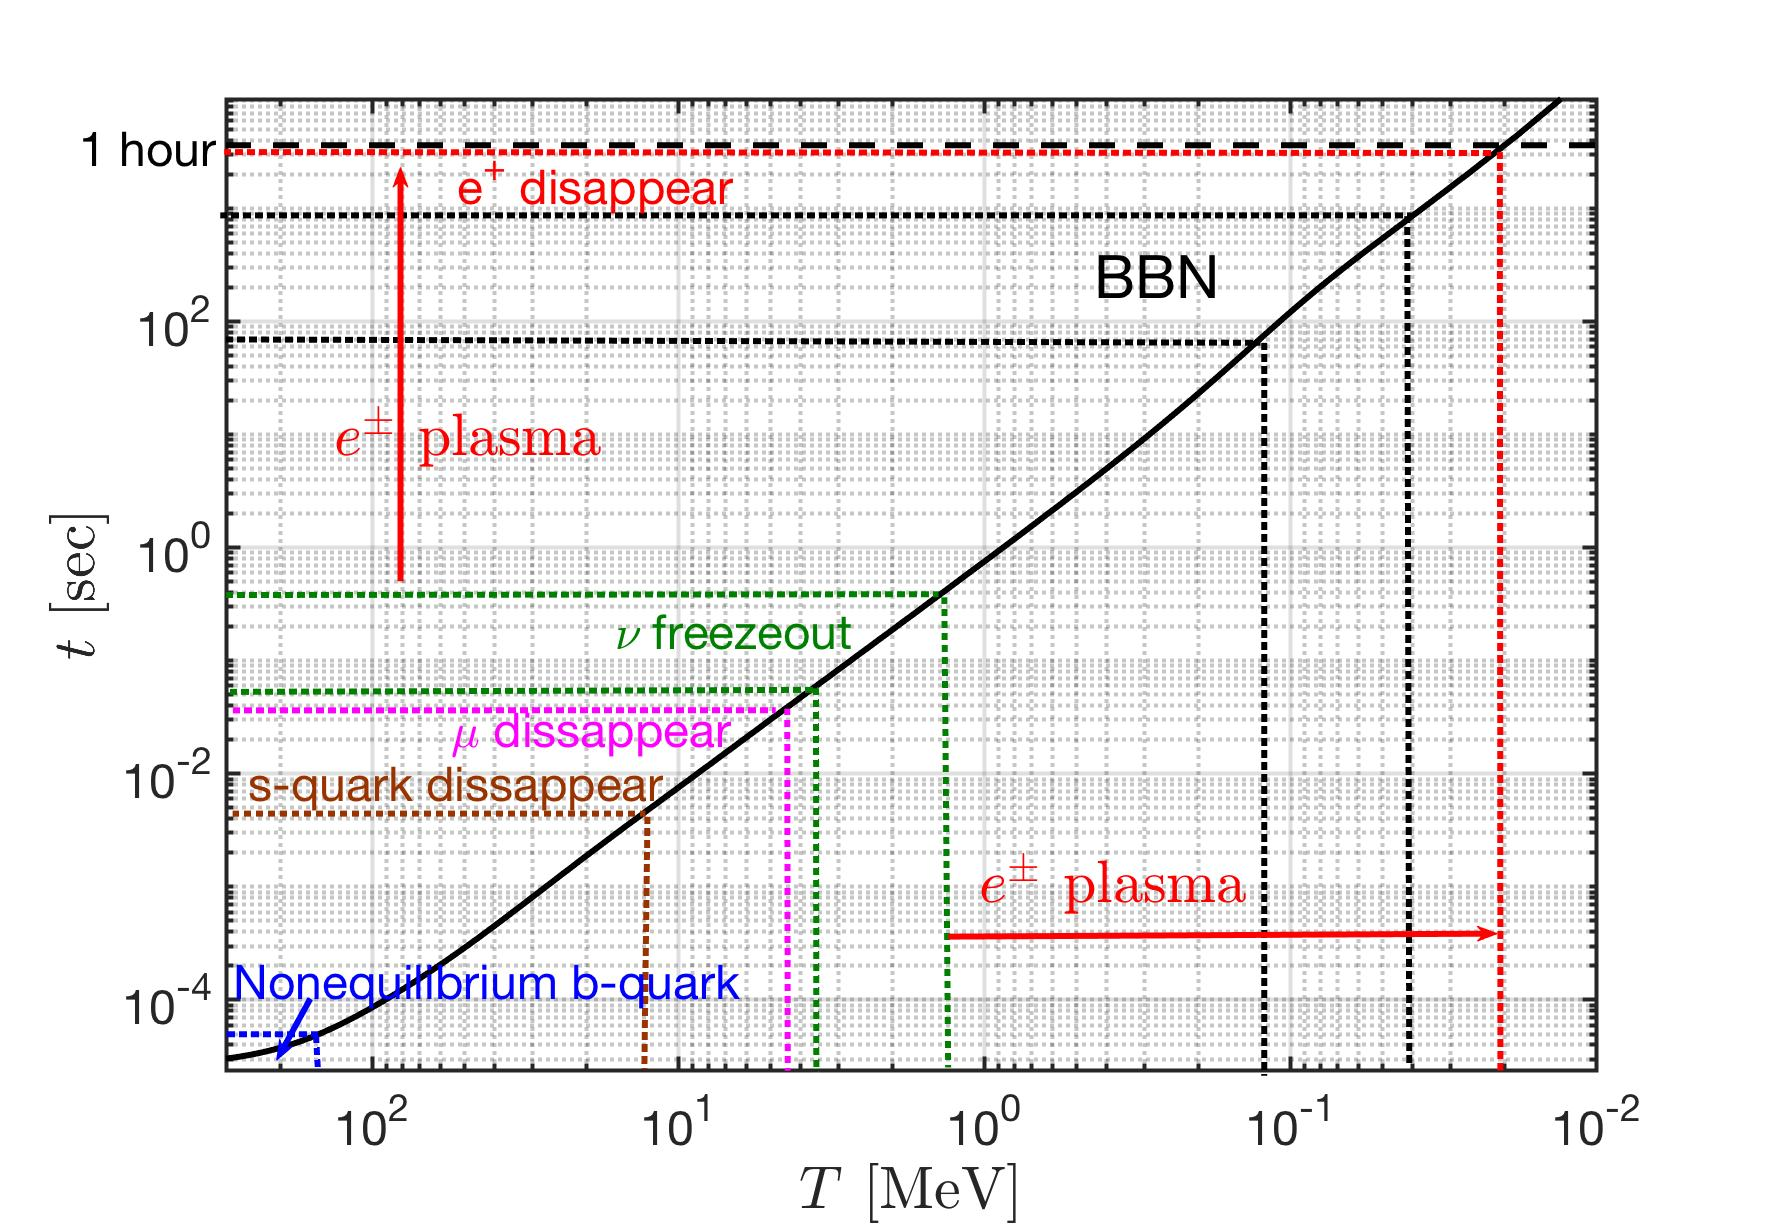
\includegraphics[width=\textwidth,width=\linewidth]{./plots/CosmicTimeTemperature_Project}}
 \caption{Adapted from the thesis of C.T. Yang \cite{Yang:2024ret}:
 The relation between time and temperature in the first hour of the Universe beginning shortly before QGP hadronization $300\,\mathrm{MeV}>T>0.02\,\mathrm{MeV} $ and ending with antimatter disappearance.Temperature/time range for several key events is indicated.}
 \label{Fig:Overview}
\end{figure}
%%%%%%%%%%%%%%%%%%%%%%%%%%%%%%%%%%%%%%%
 
We focus our study on the first hour of the Universe evolution which takes us down to temperature of about $T\simeq 20$|,keV.
\begin{enumerate}
\item \textbf{Primordial quark-gluon plasma}: 
At early times when the temperature was between $130\,\mathrm{GeV}>T>0.15\,\mathrm{GeV}$ we have the building blocks of the Universe as we know them today, including the leptons, vector bosons, and all three families of deconfined quarks and gluons which propagated freely in plasma. As all hadrons are dissolved into their constituents during this time, strongly interacting particles $u,d,s,t,b,c,g$ controlled the fate of the Universe. When temperature is near to the QGP phase transition $300\, \mathrm{MeV}>T>150$ MeV, the bottom quark breaks the detail balance and disappearance from particle inventory provides the arrow in time (see Chapter~\ref{Bottom} for detail).
 
\item \textbf{Hadronic epoch}: Around the hadronization temperature $T_H\approx150\,\mathrm{MeV}$, a phase transformation occurred, forcing the free quarks and gluons become confined within baryon and mesons \cite{Letessier:2005qe}. In the temperature range $ 150\,\mathrm{MeV}>T>20\,\mathrm{MeV}$, the Universe is rich in physics phenomena involving strange mesons and (anti)baryons including (anti)hyperon abundances~\cite{Fromerth:2012fe,Yang:2021bko}. The antibaryons disappear from the Universe at temperature $T=38.2$ MeV, and strangeness can be produced by the inverse decay reactions that are in equilibrium via weak, electromagnetic, and strong interactions in the early Universe until $T\approx13$ MeV (see Chapter~\ref{Strangeness} for detailed discussion).

\item \textbf{Lepton-photon epoch}: For temperature $10\,\mathrm{MeV}>T>2\,\mathrm{MeV}$, the Universe contained relativistic electrons, positrons, photons, and three species of (anti)neutrinos. During this epoch massless leptons and photons controlled the fate of the Universe. Massive $\tau^\pm$ disappear from the plasma at high temperature via decay processes. However $\mu^\pm$ leptons can persist in the early Universe until temperature $T=4.2$ MeV, and positron $e^+$ can persist until the temperature $T=0.02$ MeV (See Chapter~\ref{Electron} for discussion).

Neutrinos were still coupled to the charged leptons via the weak interaction~\cite{Birrell:2012gg,Birrell:2014ona} and freeze-out at temperature range $3\,\mathrm{MeV}>T>2\,\mathrm{MeV}$ which depends on the neutrino's flavors and the magnitude of the Standard Model parameters (See Chapter~\ref{Neutrino} for details). After neutrino freeze-out, they still play a important role in the Universe expansion via the effective number of neutrinos $N_{\nu}^{\mathrm{eff}}$ and affects the Hubble parameter significantly. 
\item \textbf{Electron-positron epoch}: After neutrinos freeze-out at $T=3\sim2\,\mathrm{MeV}$ and become free-streaming in the early Universe, the cosmic plasma was dominated by electrons, positrons, and photons. The $e^\pm$ plasma existed until $T\approx 0.02\,\mathrm{MeV}$. 
\item \textbf{BBN in midst of ${\mathbf e^+e^-}$ plasms:} Contrary to what was the prevailing context only a few years ago, it is today understood that BBN occurred within a rich electron-positron plasma environment. There are 1000's of${  e^+e^-}$-pairs for each nucleon undergoing nuclear BBN fusion reaction.  
\item \textbf{Primordial magnetism}\index{magnetism!primordial}: $e^{+}e^{-}$-plasma (electron-positrons pairs) at temperatures reaching well below BBN epoch in the primordial universe could be a source of the present day intergalactic magnetic fields. See Chapter~\ref{Electron} for detailed discussion. We explore Landau diamagnetic and magnetic dipole moment paramagnetic properties. A relatively small magnitude of the $e^{+}e^{-}$ magnetic moment polarization asymmetry suffices to produce a self-magnetization in the universe consistent with present day observations.
\end{enumerate}

After $e^\pm$ annihilation finishes at a temperature near 20keV, the Universe was still opaque to photons due to large scattering photon-electron Thompson cross section. Observational cosmology study ofthe Cosmic Microwave Background (CMB)~\cite{Planck:2018vyg} reaches to the epoch of free electron binding into atoms -- a process referred to as recombination -- at $T\approx 0.25\,\mathrm{eV}$. We focus on the temperature $300\,\mathrm{MeV}>T>0.02\,\mathrm{MeV}$ which corresponds to 

 We will address the cosmic plasma as follow: In Chapter~\ref{Bottom}, we discuss the heavy quarks (bottom/charm) abundance near to the QGP hadronization and show the nonequilibrium of bottom quark. In Chapter~\ref{Strangeness} we study the strangeness abundance after hadronization and show the long lasting strangeness in the early Universe. In Chapter~\ref{Neutrino} we focus on the neutrino-matter interactions and the evolution of cosmic neutrino in early universe before/after freeze-out. In Chapter~\ref{Electron} we study the abundance of charged leptons $\mu^\pm$ and $e^\pm$ and show that the present of $e^\pm$ plasma plays an important role in early Universe.
%%%%%%%%%%%%%%%%%%%%%%%%%%%%%%%%%%%%%%

%%%%%%%%%%%%%%%%%%%%%%%%%%%
\subsubsection{Quark-Gluon Plasma Epoch}
\label{sec:qgpOverview}

We will illustrate some deviations from equilibrium near to the hadronization matter formation condition. Specifically, we demonstrate the presence of chemical non-equilibrium that continues to the present day. We focus on the distinction between chemical and kinetic equilibrium and freeze-out.

We explore the following evolution of heavy strongly interacting hadrons and the annihilation of antimatter. This leads us to the leptonic dominated era in history of the Universe. Using nonquilibrium concepts, we derive those properties of neutrino freeze-out that depend only on conservation laws and are independent of the details of the microscopic scattering processes. 


...More to follow ... Include references to chapters.... jr




%%%%%%%%%%%%%%%%%%%%%%%%%%%%%%%%%%%%%%%%%
\subsubsection{Positron Antimatter}
\label{ssec:PositronView}
In the early universe during the hot dense electron-positron plasma epoch (after neutrino freeze-out), we analyze the paramagnetic characteristics of electron-positron plasma when exposed to an external primordial field. As temperature decreases nuclear reactions between remaining tiny baryon imbalance produce light nuclei and our interest in this well explored era of big-bang nucleosynthesis (BBN) is focused on the presence of a rich electron-positron plasma and its effect on nuclear reactions, a topic that has escaped wide attention. 

%%%%%%%%%%%%%%%%%%%%%%%%%%%%%%%%%%%%%%%%%
\subsubsection{Neutrino Freezeout}
\label{ssec:nuoverview}
We characterize the dependence of both $N_\nu$ and the deviation of the neutrino distribution from chemical equilibrium on the neutrino kinetic freeze-out temperature. We detail a spectral method was designed extend the regime of applicability to systems far from chemical equilibrium and/or that undergo significant reheating. 

%%%%%%%%%%%%%%%%%%%%%%%%%%%%%%%%
\subsubsection{Relic Neutrino Background}\label{ch:intro}
%{\color{blue}\textbf{CTYang:} I think this paragraph can be the introduction for cosmic neutrino background section}
At a temperature of $5$ MeV the Universe consisted of a plasma of $e^\pm$, photons, and neutrinos. At around $1$ MeV neutrinos stop interacting, or freeze-out, and begin to free-stream through the Universe. Today they comprise the relic neutrino background. Photons freeze-out around $0.25$ eV and today they make up the Cosmic Microwave Background (CMB), currently at $T_{\gamma,0}=0.235$ meV. Relic neutrinos have not been directly measured, but their impact on the speed of expansion of the Universe is imprinted on the CMB. Indirect measurements of the relic neutrino background, such as by the Planck satellite~\cite{Planck:2018vyg,Planck:2015fie,Planck:2013pxb}, constrain neutrino properties such as mass and number of massless degrees of freedom.

 In later chapters, we will study the details of the neutrino freeze-out process and their impact on observables in more detail. Here we present an overview of the era just prior to neutrino freeze-out through current epoch, putting the relic neutrinos in their proper context. Much of this material, including most Figures, was adapted from~\cite{Rafelski:2013yka}.


%%%%%%%%%%%%%%%%%%%%%%%%%%%%%%%%%%%%%%%%%%%%
\subsubsection{Reheating History of the Universe}\label{Eralink}

At times where dimensional scales are irrelevant, entropy conservation means that temperature scales inversely with the scale factor $a(t)$. This follows from \req{divTmn} when $ \rho\simeq 3P \propto T^4$. However, as the temperature drops and at their respective $m\simeq T$ scales, successively less massive particles annihilate and disappear from the thermal Universe. Their entropy reheats the other degrees of freedom and thus in the process, the entropy originating in a massive degree of freedom is shifted into the effectively massless degrees of freedom that still remain. This causes the $T\propto 1/a(t)$ scaling to break down; during each of these `reorganization' periods the drop in temperature is slowed by the concentration of entropy in fewer degrees of freedom, leading to a change in the reheating ratio, $R$, defined as
\begin{equation}\label{redshiftratio}
R\equiv \frac{1+z}{ T_\gamma/T_{\gamma,0}}, \qquad 1+z\equiv \frac{a_{0}}{a(t)}.
\end{equation}
The reheating ratio connects the photon temperature redshift to the geometric redshift, where $a_0$ is the scale factor today (often normalized to $1$) and quantifies the deviation from the scaling relation between $a(t)$ and $T$.

As we will see, the change in $R$ can be computed by the drop in the number of degrees of freedom. At a temperature on the order of the top quark mass, when all standard model particles were in thermal equilibrium, the Universe was pushed apart by 28 bosonic and 90 fermionic degrees of freedom. The total number of degrees of freedom can be computed as follows. 

For bosons we have the following: the doublet of charged Higgs particles has $4=2\times2=1+3$ degrees of freedom -- three will migrate to the longitudinal components of $W^\pm, Z$ when the electro-weak vacuum freezes and the EW symmetry breaking arises, while one is retained in the one single dynamical charge neutral Higgs component. In the massless stage, the SU(2)$\times$U(1) theory has 4$\times$2=8 gauge degrees of freedom where the first coefficient is the number of particles $(\gamma, Z, W^\pm)$ and each massless gauge boson has two transverse polarizations. Adding in $8_c\times2_s=16$ gluonic degrees of freedom we obtain 4+8+16=28 bosonic degrees of freedom. 

The count of fermionic degrees of freedom includes three $f$ families, two spins $s$, another factor two for particle-antiparticle duality. We have in each family of flavors a doublet of $2\times 3_c$ quarks, 1-lepton and 1/2 neutrinos (due left-handedness which was not implemented counting spin). Thus we find that a total $3_f\times 2_p\times 2_s\times(2\times 3_c+1_l+1/2_\nu)=90$ fermionic degrees of freedom. We further recall that massless fermions contribute 7/8 of that of bosons in both pressure and energy density. Thus the total number of massless Standard Model particles at a temperature above the top quark mass scale, referring by convention to bosonic degrees of freedom, is $g_{\rm SM}=28+90\times 7/8=106.75$ 



In \rf{fig:dof} we show the cube of the reheating ratio \req{redshiftratio} as a function of photon temperature $T_\gamma$ from the primordial high temperature early Universe on the right to the present on the left, where $R$ must be by definition unity. The periods of change seen in Figure \ref{fig:dof} come when the temperature crosses the mass of a particle species that is in equilibrium. One can see drops corresponding to the disappearance of particles as indicated. After $e^+e^-$ annihilation on the left, there are no significant degrees of freedom remaining to annihilate and feed entropy into photons, and so $R$ remains constant until today. We show the result using a Fermi gas model with a very rough model for the QGP phase transition and hadronization period near $O(100\MeV)$. The fermi gas model is a poor approximation above the QGP phase transition; a more precise model using lattice QCD, see e.g.~\cite{Borsanyi:2013bia}, together with a high temperature perturbative QCD expansion, see e.g.~\cite{Letessier:2002ony}, would be needed to improve on this situation but the details do not impact the neutrino freeze-out period near $1\MeV$ which is our primary concern, and so we do not consider these issues further here.

%%%%%%%%%%%%%%%%%%%%%%%%%%%%%%%%%%%%%%%
\begin{figure} 
\centerline{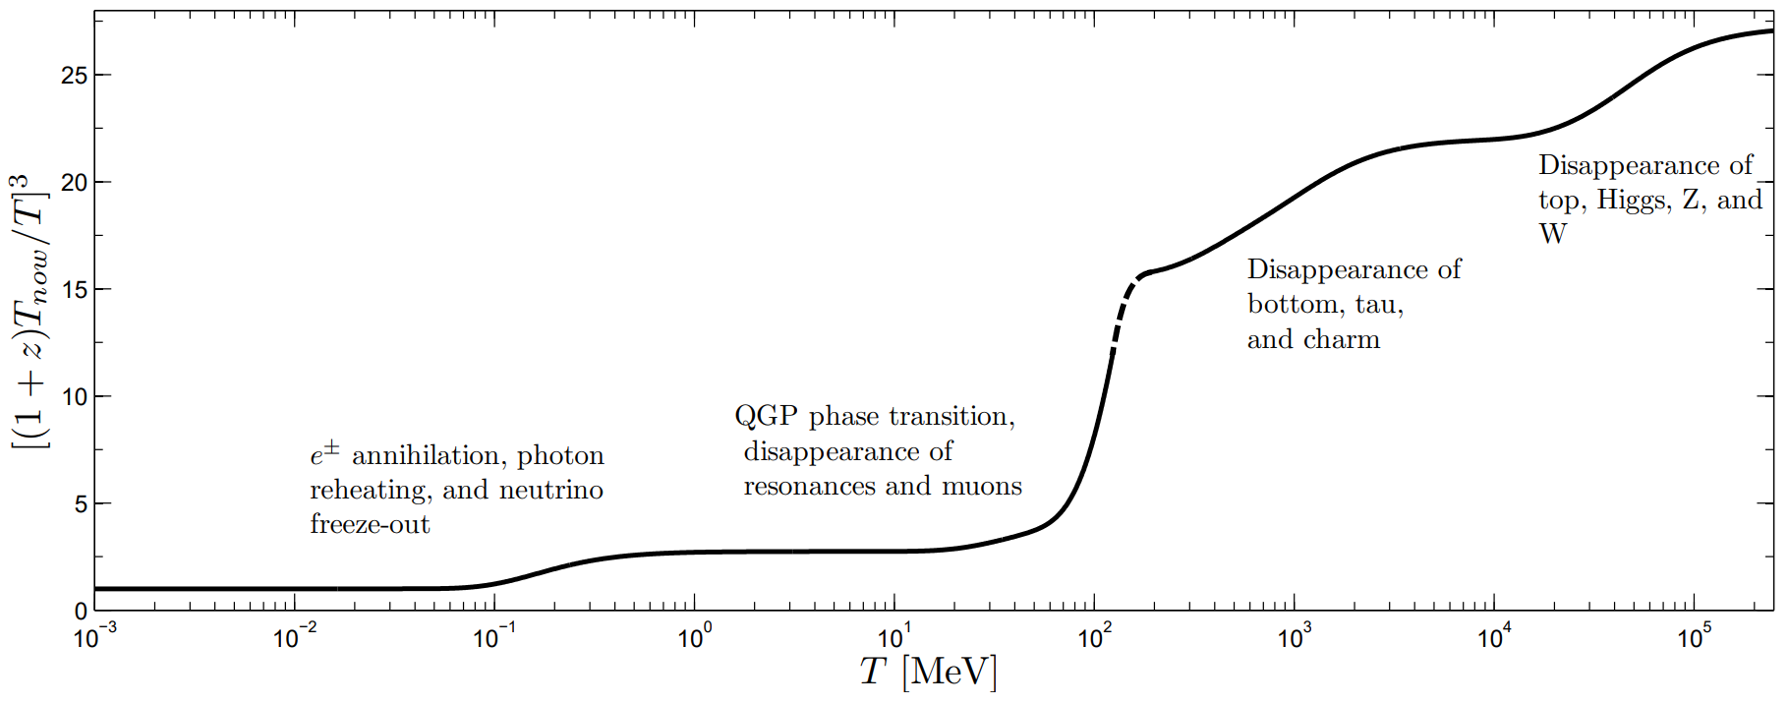
\includegraphics[height=5.2cm]{01-introduction/Figures/degrees_of_freedom.PNG}}
\caption{\cccite{Rafelski:2023emw}, adapted from Ref.~\cite{Rafelski:2013yka} and thesis of J.Birrell \cite{Birrell:2014ona}. Disappearance of degrees of freedom throughout the history of the Universe. The Universe volume inflated approximately by a factor of 27 above the thermal red shift scale as massive particles disappeared successively from the inventory. The dashed portion is a qualitative description
of QGP hadronization.\label{fig:dof}}
 \end{figure}
%%%%%%%%%%%%%%%%%%%%%%%%%%%%%%%%%%%%%%%



As long as the dynamics are at least approximately entropy conserving, the total drop in $R$ is entirely determined by entropy conservation. Namely, the magnitude of the drop in $R$ Figure~\ref{fig:dof} is a measure of the number of degrees of freedom that have disappeared from the Universe. Consider two times $t_1$ and $t_2$ at which all particle species that have not yet annihilated are effectively massless. By conservation of comoving entropy and scaling $T\propto 1/a$ we have
\begin{equation}\label{r_ratio}
1=\frac{a_1^3S_{1}}{a_2^3 S_2}=\frac{a_1^3\sum_ig_i T_{i,1}^3}{a_2^3\sum_j g_j T_{j,2}^3},\qquad \left(\frac{R_1}{R_2}\right)^3=\frac{\sum_ig_i (T_{i,1}/T_{\gamma,1})^3}{\sum_j g_j (T_{j,2}/T_{\gamma,2})^3}
\end{equation}
where the sums are over the total number of degrees of freedom present at the indicated time and the degeneracy factors $g_i$ contain the $7/8$ factor for fermions. In the second form we divided the numerator and denominator by $a_{0}T_{\gamma,0}$. We distinguish between the temperature of each particle species and our reference temperature, the photon temperature. This is important since today neutrinos are colder than photons, due to photon reheating from $e^\pm$ annihilation occurring after neutrinos decoupled (this is only an approximation, a point we will study in detail in subsequent chapters). By conservation of entropy one obtains the neutrino to photon temperature ratio of
\begin{equation}\label{T_nu_T_gamma}
T_\nu/T_\gamma=({4}/{11})^{1/3}.
\end{equation}
We will call this the reheating ratio in the decoupled limit. For details on the derivation of this standard result, see, e.g., Section \ref{Tnugam} where it is obtained as a special case of a more general analysis.

Using \req{r_ratio} we compute the total drop in $R^3$ shown in Figure \ref{fig:dof}. At $T=T_\gamma=\mathcal{O}(100\GeV)$ the number of active degrees of freedom is slightly below $g_{\rm SM}=106.75$ due to the partial disappearance of top quarks, but this approximation will be good enough for our purposes. At this time, all the species are in thermal equilibrium with photons and so $T_{i,1}/T_{\gamma,1}=1$ for all $i$. Today we have $2$ photon and $7/8\times 6$ neutrino degrees of freedom and a neutrino to photon temperature ratio \req{T_nu_T_gamma}. Therefore we have
\begin{equation}
\left(\frac{R_{100GeV}}{R_{now}}\right)^3= \frac{g_{SM}}{g_{\rm now}}=\frac{106.75}{2+\frac{7}{8}\times 6\times \frac{4}{11}}\approx 27.3
\end{equation}
which is the fractional change we see in the fermi gas model curve in Figure \ref{fig:dof} (as mentioned above, the QCD model is reduced due to interactions). The meaning of this factor is that the Universe approximately inflated by a factor 27 above the thermal red shift scale as massive particles disappeared successively from the inventory. 

From the perspective of reheating, the history of the Universe from the end of $e^\pm$ annihilation until today has been uneventful. 

We can shed additional light on this period and others by looking at the composition of the Universe as a function of temperature

%%%%%%%%%%%%%%%%%%%%%%%%%%%%%%%%%%%%
\begin{figure}
\centerline{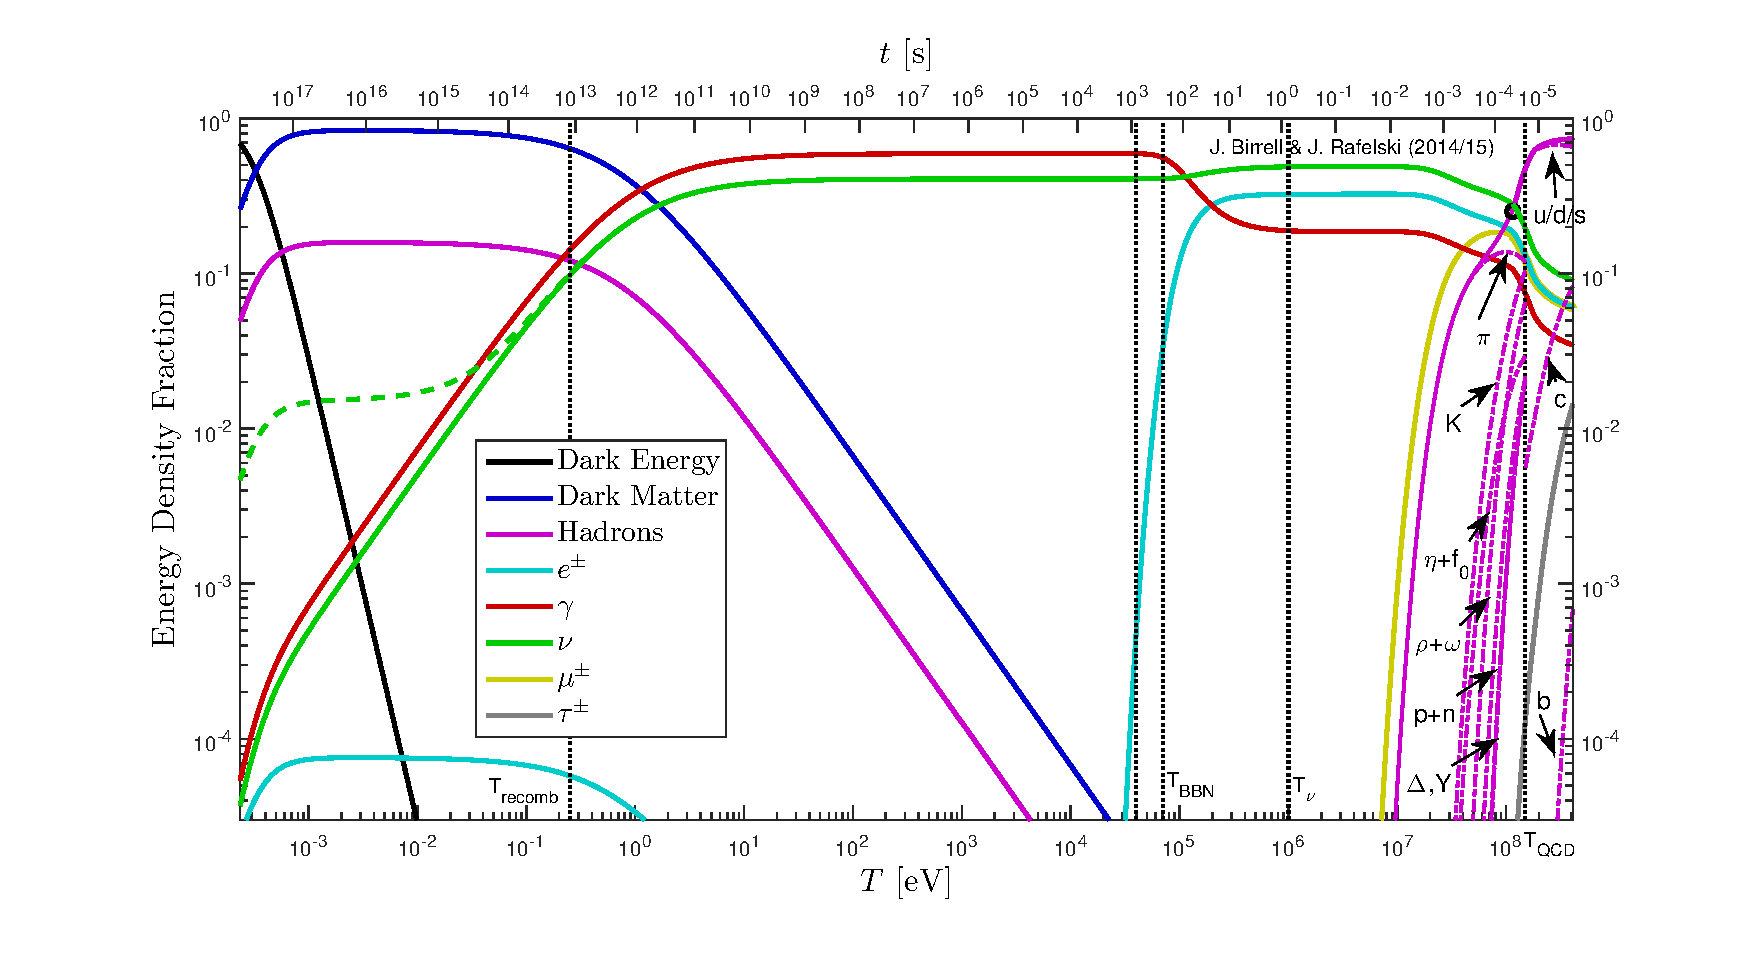
\includegraphics[height=8.2cm]{01-introduction/Figures/energy_densities_total.eps}}\label{fig:energy_frac}
\caption{\cccite{Rafelski:2023emw}, expanded from results of the thesis of J.Birrell \cite{Birrell:2014ona}. Current era: $69\%$ dark energy, $26\%$ dark matter, $5\%$ baryons, $<1\%$ photons and neutrinos, $1$ massless and $2\times .1$ eV neutrinos (Neutrino mass choice is just for illustration. Other values are possible). }
 \end{figure}
%%%%%%%%%%%%%%%%%%%%%%%%%%%%%%%%%%
In Figure \ref{fig:energy_frac} we begin on the right at the end of the hadron era with the disappearance of muons and pions. This constitutes a reheating period, with energy and entropy from these particles being transferred to the remaining $e^\pm$, photon, neutrino plasma. Continuing to $T=O(1)$ MeV, we come to the annihilation of $e^\pm$ and the photon reheating period. Notice that only the photon energy density fraction increases here. As discussed above, a common simplifying assumption is that neutrinos are already decoupled at this time and hence do not share in the reheating process, leading to a difference in photon and neutrino temperatures \req{T_nu_T_gamma}.

After passing through a long period, from $T=O(1)$ MeV until $T=O(1)$ eV, where the energy density is dominated by photons and free-streaming neutrinos, we then come to the beginning of the matter dominated regime, where the energy density is dominated by dark matter and baryonic matter. This transition is the result of the redshifting of the photon and neutrino energy, $\rho\propto T^4$, whereas for non-relativistic matter $\rho\propto a^{-3}\propto T^3$. Note that our inclusion of neutrino mass causes the leveling out of the neutrino energy density fraction during this period, as compared to the continued redshifting of the photon energy.

Finally, as we move towards the present day CMB temperature of $T_{\gamma,0}=0.235$ meV on the left hand side, we have entered the dark energy dominated regime. For the present day values, we have used the fits from the Planck data~\cite{Planck:2018vyg,Planck:2015fie,Planck:2013pxb} of $69\%$ dark energy, $26\%$ dark matter and $5\%$ baryons (and zero spatial curvature). The photon energy density is fixed by the CMB temperature $T_{\gamma,0}$ and the neutrino energy density is fixed by $T_{\gamma,0}$ along with the photon to neutrino temperature ratio. Both constitute $<1\%$ of the current energy budget.

%%%%%%%%%%%%%%%%%%%%%%%%%%%%%%%%%%%%%%%%%%%%%%
%\subsubsection\label{recomb}
\paragraph{Back in time to Neutrino Freeze-out:}
In the following we use the mix of matter (31\%) and dark energy (69\%) with photon and neutrino backgrounds favored by the latest Planck results~\cite{Planck:2018vyg,Planck:2015fie,Planck:2013pxb}, where we gave two neutrino species mass of $m_\nu=30\meV$ and a third neutrino remains massless. This is a different mass value than used above and again, it is only for illustration-- other mass choices are possible within present day constraints and will impact to some degree where exactly matter dominance emerges from the radiative Universe. We presume that neutrino kinetic freeze-out completed before the onset of $e^\pm$-annihilation into photons, leading to the neutrino to photon temperature ratio \req{T_nu_T_gamma}. Again, this is a common simplifying assumption. Much of the remainder of this work will involve improving on this approximation, but for the purposes of this overview it is sufficient.

Figure \ref{fig:today} shows in the left frame the temperature (left axis) and deceleration parameter (right axis) from shortly after the completion neutrino freeze-out until today. The horizontal dot-dashed lines show the pure radiation-dominated value of $q=1$ and the matter-dominated value of $q=1/2$. The expansion in this era starts off as radiation-dominated, but transitions to matter-dominated starting around $T=\mathcal{O}(10\eV)$ and begins to transition to a dark energy dominated era at $T=\mathcal{O}(1\meV)$. We are still in the midst of this transition today. The vertical dot-dashed lines show the time of recombination at $T\simeq0.25\eV$, when the Universe became transparent to photons, and reionization at $T\simeq {\cal O}(1\meV)$, when hydrogen in the Universe was again ionized due to light from the first galaxies~\cite{Zaroubi:2012in}. 

On the right in Figure \ref{fig:today} we show the Hubble parameter $H$ and redshift $z+1\equiv a_0/a(t)$. We can see in Figure \ref{fig:today} a visible deviation from power law behavior due to the transitions from radiation to matter dominated and from matter to dark energy dominated expansion. These transitions are accentuated and more easily visualized in the form of the deceleration parameter $q$. The time span covered by the Figure \ref{fig:today} is in essence the entire lifespan of the Universe, but of course on a logarithmic time scale there is a lot of room for interesting physics in the tiny blip that happened beforehand.


%%%%%%%%%%%%%%%%%%%%%%%%%%%%%%%%%%%%%%%
\begin{figure}
\begin{minipage}{\linewidth}
\makebox[0.5\linewidth]%
{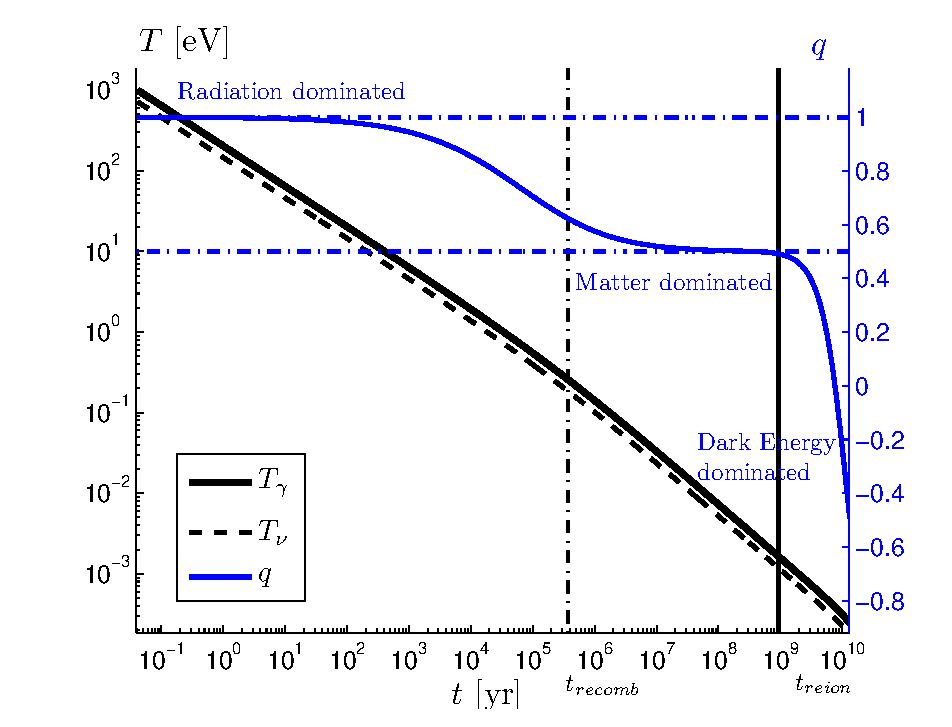
\includegraphics[keepaspectratio=true,scale=0.52]{01-introduction/Figures/T_q_today.eps}}
\makebox[0.5\linewidth]%
{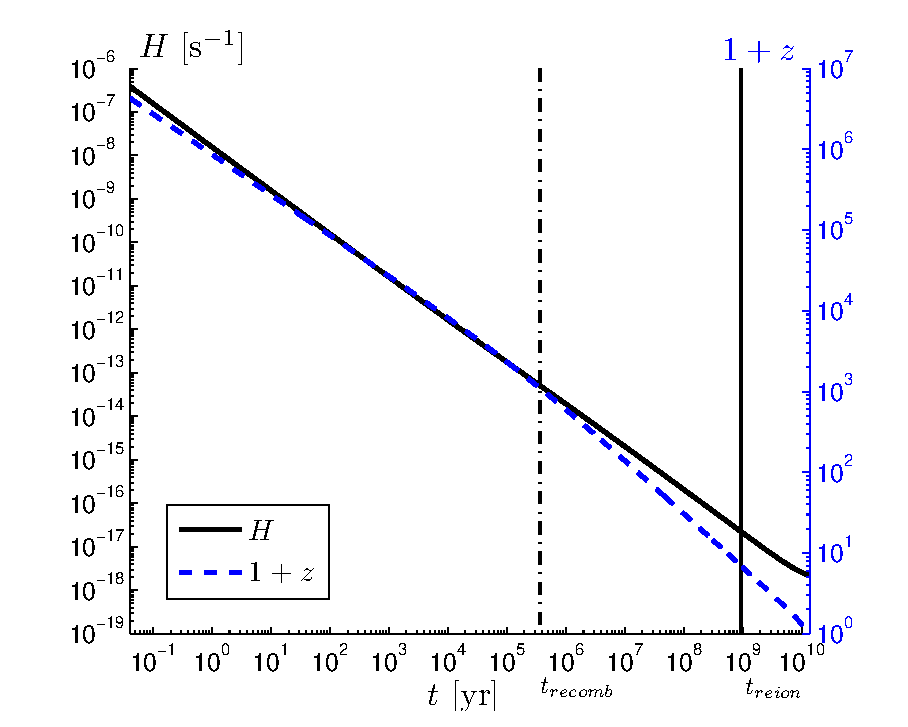
\includegraphics[keepaspectratio=true,scale=0.52]{01-introduction/Figures/H_z_today.eps}}
\caption{\cccite{Rafelski:2013yka}: Transition periods in the composition of the Universe: on left -- evolution of temperature $T$ and deceleration parameter $q$; on right -- evolution of the Hubble parameter $H$ and redshift $z$. 
\label{fig:today} }
\end{minipage}
\end{figure}
%%%%%%%%%%%%%%%%%%%%%%%%%%%%%%%%%%%%%%%

%%%%%%%%%%%%%%%%%%%%%%%%%%%%%%%%%%%%%%%%%
\subsubsection{Neutrino freeze-out era} \label{nudecoup}
%\paragraph{Neutrino freeze-out era:} 
The era separating the photon-neutrino-matter-dark energy Universe we just described from the end of the hadron Universe is quite complex in its evolution. We begin when the number of $e^\pm$-pairs has decayed to the same abundance as the number of baryons in the Universe at the temperature $T=\mathcal{O}(10\keV)$ and reach back to $T={\cal O}(30\MeV)$ where muons and pions are disappearing from the Universe.

%%%%%%%%%%%%%%%%%%%%%%%%%%%%%%%%%%%%%%%
\begin{figure}
\begin{minipage}{\linewidth}
\makebox[0.5\linewidth]%
{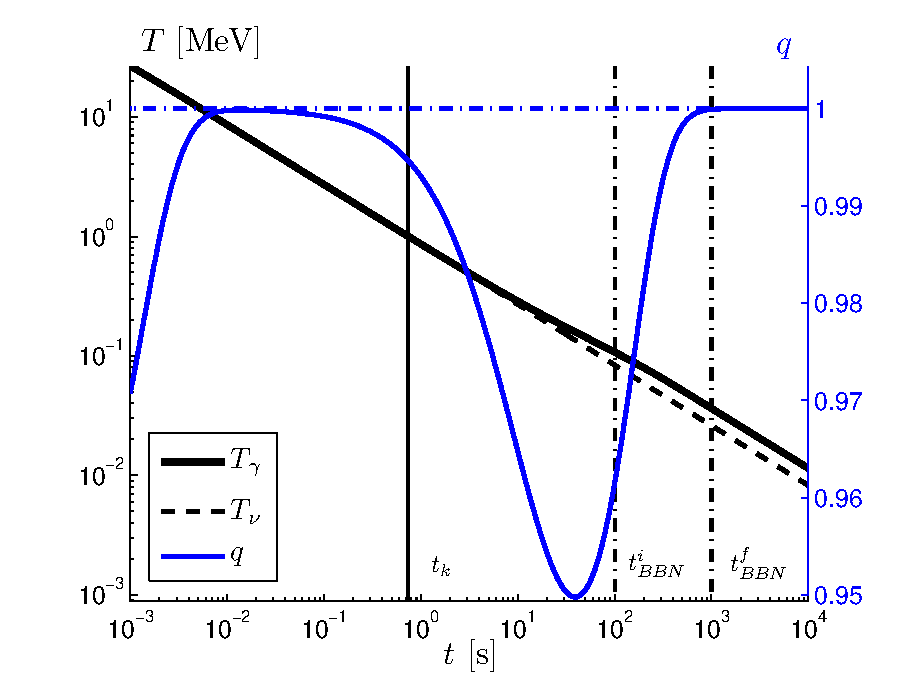
\includegraphics[keepaspectratio=true,scale=0.54]{01-introduction/Figures/T_q_BBN.eps}} 
\makebox[0.5\linewidth]%
{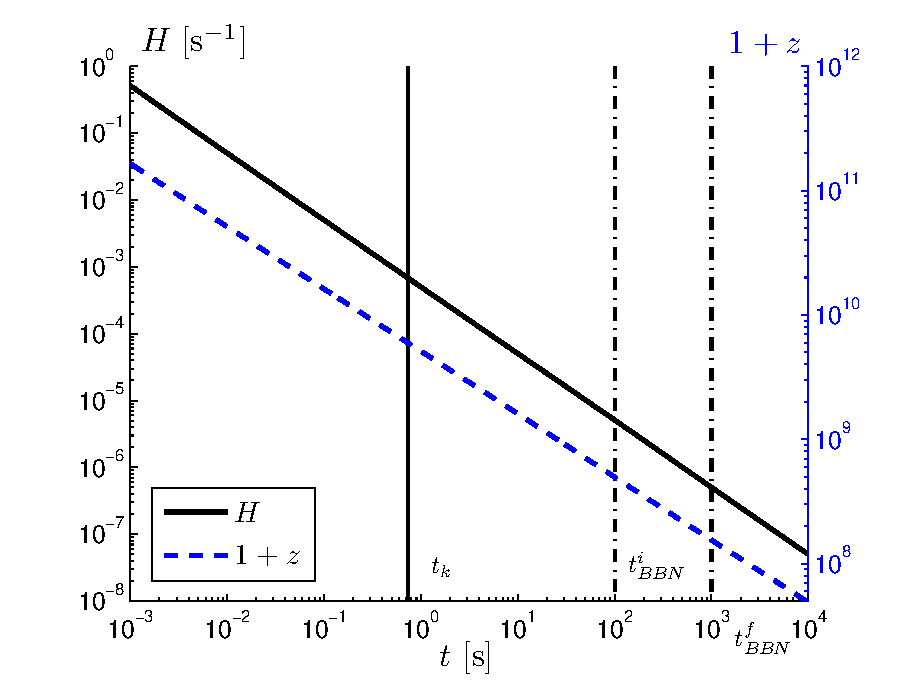
\includegraphics[keepaspectratio=true,scale=0.54]{01-introduction/Figures/H_z_BBN.eps}} 
\caption{\cccite{Rafelski:2013yka}: From the end of baryon antimatter annihilation through BBN, see Figure \ref{fig:today}. % on left -- evolution of temperature $T$ and deceleration parameter $q$; on right -- evolution of the Hubble parameter $H$ and redshift $z$.
\label{fig:BBN} }
\end{minipage}
\end{figure}
%%%%%%%%%%%%%%%%%%%%%%%%%%%%%%%%%%%%%%%

 In Figure~\ref{fig:BBN} the horizontal dot-dashed line for $q=1$ shows the pure radiation dominated value with two exceptions. First, the presence of massive pions and muons reduce the value of $q$ near to the maximal temperature shown. Second, when the temperature is near the value of the electron mass, the $e^\pm$-pairs are not yet fully depleted but already sufficiently non-relativistic to cause another dip in $q$. These are not large drops; the expansion is still predominately radiation dominated. But $q$ provides a sensitive measure of when various mass scales become relevant and is a good indicator of the presence of a reheating period.

 The dashed line shows the neutrino temperature, which decouples from the $e^\pm$ and photon temperature at $T={\cal O}(1\MeV)$ when neutrinos freeze-out and begin free streaming. In Figure~\ref{fig:BBN} the unit of time is seconds and the range spans the domain from fractions of a millisecond to a few hours. After neutrino freeze-out we come to Big Bang Nucleosynthesis, the period when the lighter elements were synthesized in a hot but relatively dilute plasma~\cite{Iocco:2008va}. We left some time gap between this and the domain shown in Figure \ref{fig:today} describing the current era -- there is an uneventful evolution between the two domains. 
 


%%%%%%%%%%%%%%%%%%%%%%%%%%%%%%%%%%%%%%%%%%%%%%%%%
\subsubsection{Overview of neutrino freeze-out in the early Universe}
 Neutrino freeze-out is, as far as we know, the unique era in the history of the Universe when a significant matter fraction froze out at the same time that a reheating period was beginning, namely the start of $e^\pm$ annihilation. It is this coincidence that makes neutrino freeze-out a rich and complicated period to study as compared to the many other reheating periods in the history of the Universe. 

The properties of the neutrino background are influenced by the details of the freeze-out or decoupling process at a temperature $T=\mathcal{O}(2\mathrm{MeV})$. In the literature one finds estimates of freeze-out temperatures based on a comparison of Hubble expansion with neutrino scattering length and considering only number changing (i.e. chemical) processes. In the paper~\cite{Birrell:2014uka}, we employ a similar definition of freeze-out temperature in the context of the Boltzmann equation and refine the results by noting that there are three different freeze-out processes for neutrinos:

%In general, the particle freezeout process include both chemical and kinetic which lead to particle become free-streaming in the early Universe (for detail discussion see Chapter~\ref{Introduction}), we have:

1. Neutrino chemical freeze-out: the temperature at which neutrino number changing processes such as $e^-e^+\to\nu\overline\nu$ effectively cease. After chemical freeze-out, there are no reactions that, in a noteworthy fashion, can
change the neutrino abundance and so particle number is conserved. %Prior to the chemical freezeout temperature, number changing processes are significant and keep the particle in chemical (and thermal) equilibrium, implying the distribution function of neutrino has the Fermi-Dirac form:
%\begin{equation}\label{equilibrium}
%f_{c}(t,E)=\frac{1}{\exp(E/T)+1}, \qquad\text{ for } T> T_{ch}.
%\end{equation}

2. Neutrino kinetic freeze-out: the temperature at which the neutrino momentum exchanging interactions such as $e^\pm\nu\to e^\pm\nu$ are no longer occurring rapidly enough to maintain an equilibrium momentum distribution. %When $T_k<T(t)<T_{ch}$, the number-changing process no longer occurs rapidly enough to keep the distribution in chemical equilibrium but there is still sufficient momentum exchange to keep the distribution in thermal equilibrium. The distribution function is therefore obtained by maximizing entropy, with fixed energy, particle number, and antiparticle number separately. This implies that the distribution function has the form
%\begin{equation}\label{kinetic_equilib}
%f_k(t,E)=\frac{1}{\Upsilon^{-1}\exp(E/T)+1},\qquad \text{ for }T_k< T< T_{ch}.
%\end{equation}
%The time dependent generalized fugacity $\Upsilon(t)$ controls the occupancy of phase space and is necessary once $T(t)<T_{ch}$ in order to conserve particle number.

3. Collisions between neutrinos:
Those collisions $\nu\nu\to\nu\nu$ are capable of reequilibrating energy within and between neutrino flavor families. These processes end at a yet lower temperature and the neutrinos will be truly free-streaming from that point on.
 
%3. Free streaming: for $T<T_k$ there are no longer any significant interactions that couple the particle species of interest and so they begin to free-stream through the Universe. The Einstein-Vlasov equation can be solved~\cite{Choquet-Bruhat:2009xil,Birrell:2012gg}, to yield the free-streaming momentum distribution
%\begin{equation}\label{free_stream_dist}
%f(t,E)=\frac{1}{\Upsilon^{-1}e^{\sqrt{p^2/T_{fs}^2+m_\nu^2 /T_k^2}}+ 1},\qquad T_{fs}=\frac{T_ka(t_k)}{a(t)}
%\end{equation}
%where the free-streaming effective temperature $T_{fs}$ is obtained by redshifting the temperature at kinetic freeze-out, and $m_\nu$ is the mass of neutrino.





To estimate the freeze-out temperature, we need to solve the Boltzmann equation with different types of collision terms with the transition matrices from Table.~\ref{T005} and Table.~\ref{T006}. The paper~\cite{Birrell:2014uka} developed a new method for analytically simplifying the collision integrals and showing that the neutrino freeze-out temperature is controlled by fundamental coupling constants and particle masses. The freeze-out temperature depends only on the magnitude of the Weinberg angle in the form $\sin^2(\theta_W)$, and a dimensionless relative interaction strength parameter $\eta$,
\begin{align}
\eta\equiv M_p m_e^3 G_F^2, \qquad M_p^2\equiv \frac{1}{8\pi G_N}, \end{align}
a combination of the electron mass $m_e$, Newton constant $G_N$ (expressed above in terms of Planck mass $M_p$), and the Fermi constant $G_F$. The dimensionless interaction strength parameter $\eta$ in the present-day vacuum has the value
\begin{align}
\eta_0\equiv \left.M_p m_e^3 G_F^2\right|_0 = 0.04421 .
\end{align}

The magnitude of $\sin^2(\theta_W)$ is not fixed by known phenomena. It could be subject to variation as a function of time or temperature. In \rf{fig:freezeoutT} we show the dependence of neutrino freeze-out temperatures for $\nu_e$ and $\nu_{\mu,\tau}$ on SM model parameters $\sin^2(\theta_W)$ and $\eta$ in detail. We note the difference in freeze-out between electron neutrino and the heavier flavors. However:

 
%~~~~~~~~~~~~~~~~~~~~~~~~~~~~~~~~~~~~~~~~~~~~~~~~~
\begin{figure}[ht]
\centerline{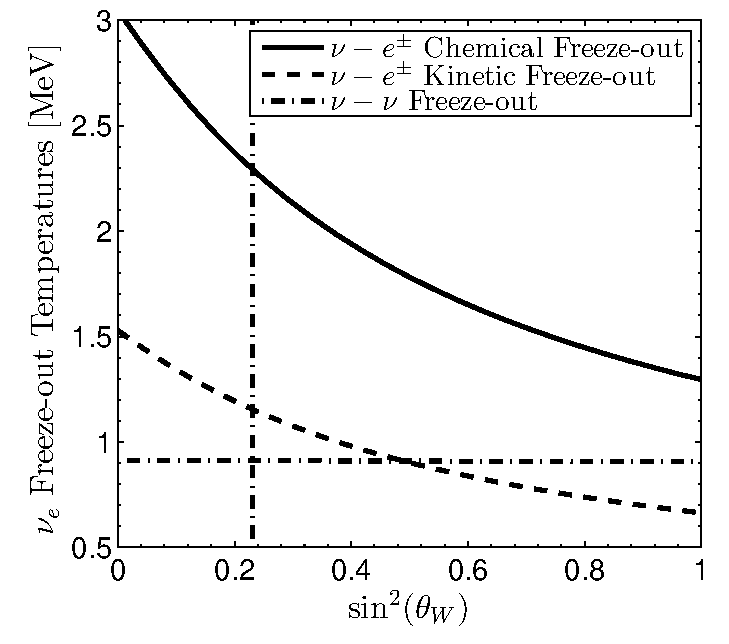
\includegraphics[width=0.47\columnwidth]{./plots/nu_e_freezeout.pdf}
\hspace{1mm}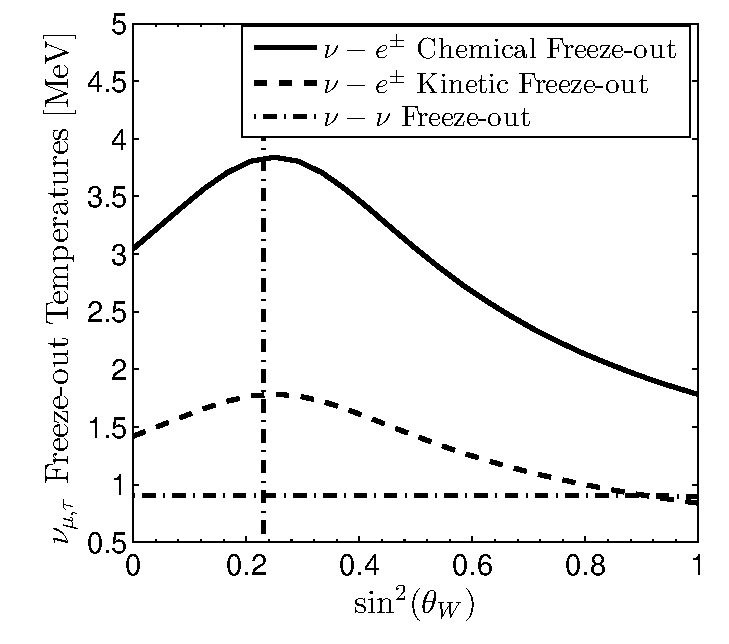
\includegraphics[width=0.47\columnwidth]{./plots/nu_mu_freezeout.pdf}}
\centerline{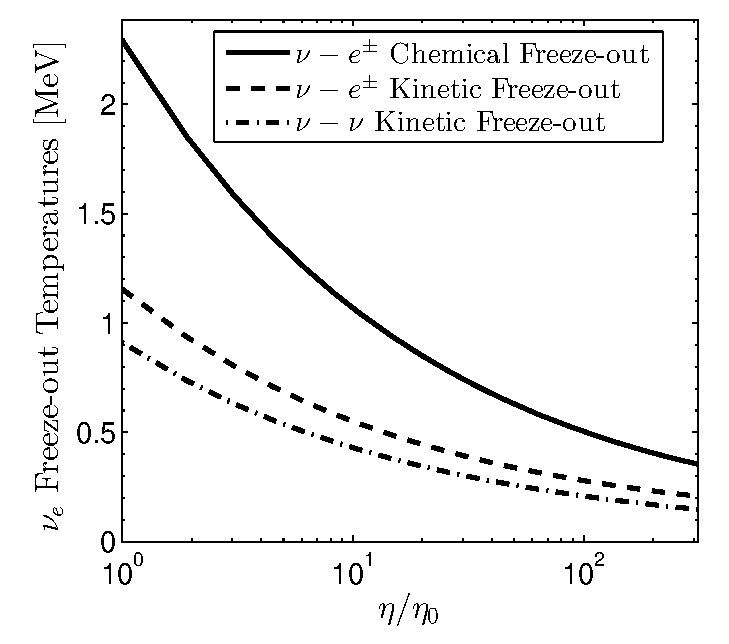
\includegraphics[width=0.47\columnwidth]{./plots/nu_e_freezeout_GF.pdf}
\hspace{1mm}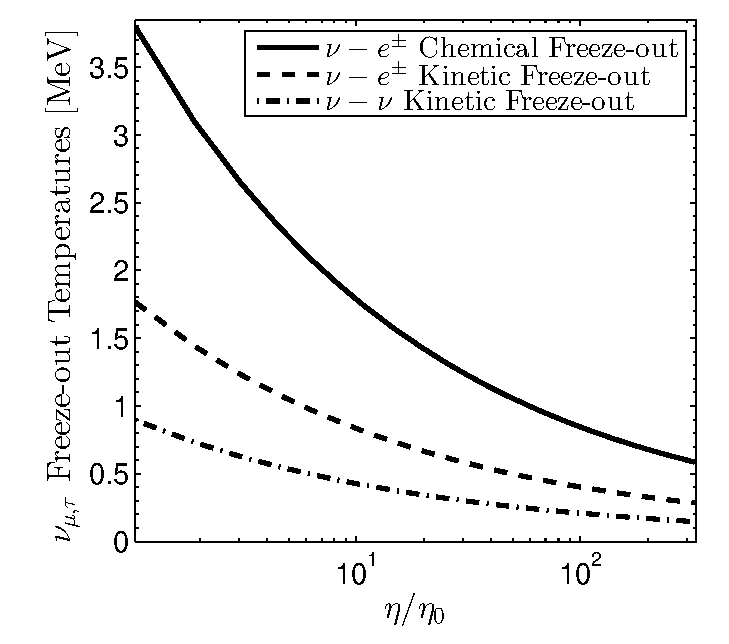
\includegraphics[width=0.47\columnwidth]{./plots/nu_mu_freezeout_GF.pdf}}

\caption{\cccite{Birrell:2014uka}, adapted from Ref.~\cite{Birrell:2014uka} and thesis of J.Birrell \cite{Birrell:2014ona}. Freeze-out temperatures for electron neutrinos (left) and $\mu$, $\tau$ neutrinos (right) for the three types of freeze-out processes. Top panels print temperature curves as a function of $\sin^2(\theta_W)$ for $\eta=\eta_0$, the vertical dashed line is $\sin^2(\theta_W)=0.23$; bottom panels are printed as a function of relative change in interaction strength $\eta/\eta_0$ obtained for $\sin^2(\theta_W)=0.23$.}
\label{fig:freezeoutT}
 \end{figure}
%~~~~~~~~~~~~~~~~~~~~~~~~~~~~~~~~~~~~~~~~~~~~~

Neutrinos are produced in elementary processes in flavor eigenstates. These are not mass eigenstates. Due to the difference in neutrino mass the coherent propagating components move at different velocity. Their very, very low interaction probability creates in laboratory the effect one refers to as `flavor oscillation'. How does this impact neurino freeze-out? Near to freeze-out temperature the electron-neutrino can still `annihilate' on electrons while absence of muons and taus in the cosmic plasma at a temperature of a few MeV makes these two neutrino flavors less interactive. 

Oscillation thus provide a mechanism in which the heavier flavors remain reactive in matter as they develop the more interactive electron-neutrino component. Conversely, electron neutrino freeze-out is occurring sooner than presented in \rf{fig:freezeoutT} since only a part of this flavor wave remains available to interact. Overall the difference in freeze-out of the three different flavors diminishes compared to results seen in \rf{fig:freezeoutT}. However, the effect was found negligible in work of Mangano et. al.~\cite{Mangano:2005cc}.

A discussion of the implications and connections of the results on neutrino freezeout to other areas of physics, including Big Bang Nucleosynthesis and dark radiation is described in more detail in~\cite{Dreiner:2011fp,Boehm:2012gr,Blennow:2012de,Birrell:2014uka}. A comprehensive investigation of neutrino freezeout, and a novel approach to analytically simplify the collision integrals for the Boltzmann equation can be found in Jeremiah Birrell‘s PhD thesis~\cite{Birrell:2014ona}. 

%%%%%%%%%%%%%%%%%%%%%%%%%%%%%%%%%%%%%%%%%%%%%%%
\subsubsection{Electron-positron plasma during BBN}\label{sec:density}
In this section, we will review the presence of electron-positron plasma during BBN. Before BBN, temperatures $T>86.7\,$keV were high enough that any nuclei formed would be disassociated by the vast number of high energy photons present \cite{Pitrou:2018cgg}. Once the temperature cooled to around $T<50\,$keV most of the nuclear reactions forming nuclei had already occurred. In this study, we can neglect the universe's expansion since, at this period, the time scale of expansion $H^{-1}$ is orders of magnitude larger than the time scale of BBN. We also note that at this point neutrinos have become free streaming \cite{Birrell:2012gg}.

In \cite{Grayson:2022asf}, C.T. Yang used the present-day baryon-to-photon ratio: $B/N_\gamma =n_B/n_\gamma= 6.05\times10^{-10}$ from Cosmic Microwave Background (CMB)~\cite{ParticleDataGroup:2022pth} and the charge neutrality of the universe to find the electron-positron chemical potential and density during BBN.

\begin{figure}[ht]
\begin{center}
%\includegraphics[width=0.95\linewidth]{Chemical_Plasma}
%\includegraphics[width=0.95\linewidth]{Density_Plasma002}
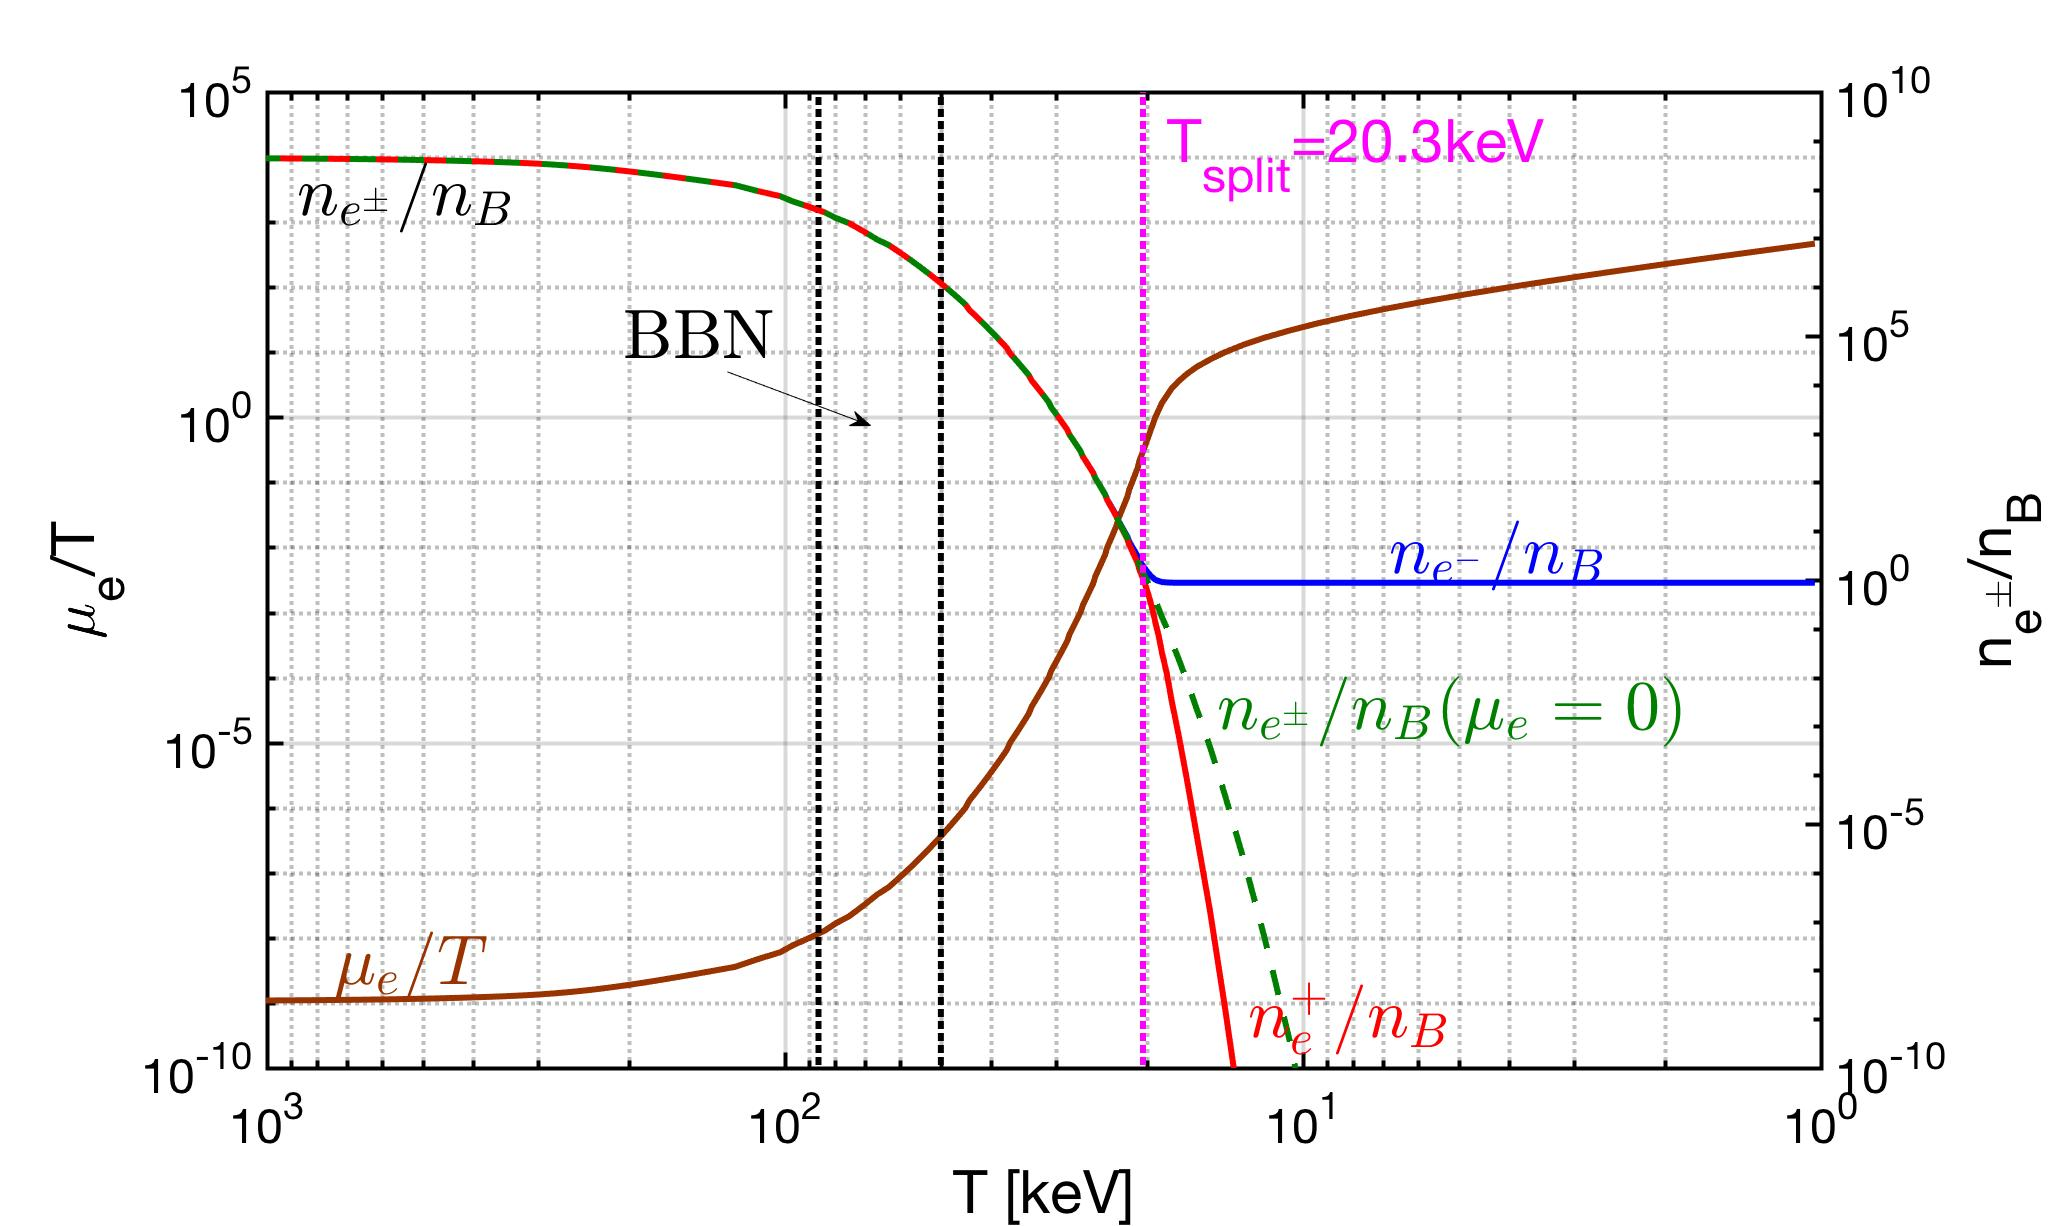
\includegraphics[width=0.95\linewidth]{plots/chap03BBN/May152023_EPDensity_Chemical}
\caption{\cccite{Grayson:2023flr}, adapted from Ref.~\cite{Grayson:2023flr} and thesis of C.T.Yang \cite{Yang:2024ret}. Left axis: The chemical potential of electrons as a function of temperature. Right axis: the ratio of electron (positron) number density to baryon density as a function of temperature. The solid blue line is the electron density, the red dashed line is the positron density, and the green dotted line is the number density with $\mu_e=0$. When $T=20.3\,\mathrm{keV}$ (the purple vertical line) positron density decreases rapidly because of the annihilation. The vertical black dotted lines represent BBN temperature range $86\,\mathrm{keV}>\mathrm{T_{BBN}}>50\,\mathrm{keV}$.}
\label{BBN_Electron}
\end{center}
\end{figure}

In Fig.~\ref{BBN_Electron} (left axis), we plot the electron chemical potential as a function of temperature. We can see the value of chemical potential is comparatively small $\mu_e/T\approx10^{-6}\sim10^{-7}$ during the BBN temperature range, implying an equal number of electrons and positrons in plasma. Thus, for the proceeding calculations, we will set $\mu =0$. When the temperature is around $T=70\,\mathrm{keV}$, the density of electrons and positrons is comparatively large $n_{e^\pm}\approx10^7\,n_B$. This indicates that we can assume the universe is filled mainly with electrons and positrons with light nuclei being a very small component of the plasma. Later when the temperature is around $T=20.3\,\mathrm{keV}$, the positron density decreases, transforming the pair-plasma to an electron-baryon plasma.


% In this section, we will derive the dependence of electron chemical potential, and hence $e^+e^-$ density, as a function of the photon background temperature $T$ by employing the following physical principles:
% \begin{enumerate}
% \item Charge neutrality of the Universe:
% \begin{align}\label{neutrality}
% n_{e^-}-n_{{e^+}}=n_p-n_{\overline{p}}\approx\,n_p,
% \end{align}
% where $n_\ell$ denotes the number density of particle type $\ell$.
% \item Neutrinos decouple (freeze out) at a temperature $T_f\simeq 2$ MeV, after which they free stream through the Universe with an effective temperature~\cite{Birrell:2012gg}
% \begin{align}
% T_\nu(t)=T_f\,\frac{a(t_f)}{a(t)},
% \end{align}
% where $a(t)$ is the--Friedmann--Lema\^{i}tre--Robertson--Walker (FLRW) Universe scale factor which is a function of cosmic time $t$, and $t_f$ represents the cosmic time when neutrino freezes out.
% \item Total comoving entropy is conserved. At $T\leq T_f$, the dominant contributors to entropy are photons, $e^+e^-$, and neutrinos. In addition, after neutrino freeze out, neutrino comoving entropy is independently conserved~\cite{Birrell:2012gg}. This implies that the combined comoving entropy in $e^+e^-\gamma$ is also conserved for $T\leq T_f$.
% \end{enumerate}

% Motivated by the fact that comoving entropy in $\gamma$, $e^+e^-$ is conserved after neutrino freezeout, we rewrite the charge neutrality condition, Eq.~(\ref{neutrality}), in the form
% \begin{align}\label{charge_neutral_cond2}
% n_{e^-}-n_{{e^+}}=X_p\frac{n_B}{s_{\gamma,e^\pm}} s_{\gamma,e^\pm},\qquad X_p\equiv\frac{n_p}{n_B},
% \end{align}
% where $n_B$ is the number density of baryons, $s_{\gamma,e^\pm}$ is the combined entropy density in photons, electrons, and positrons. During the Universe expansion, the comoving entropy and baryon number are conserved quantities; hence the ratio $n_B/s_{\gamma,e^\pm}$ is conserved. We have
% \begin{align}
% \frac{n_B}{s_{\gamma,e^\pm,}}=\left(\frac{n_B}{s_{\gamma,e^\pm}}\right)_{t_0}\!\!\!\!=\left(\frac{n_B}{s_{\gamma}}\right)_{t_0}\!\!\!\!=\left(\frac{n_B}{n_\gamma}\right)_{t_0}\left(\frac{n_\gamma}{s_{\gamma}}\right)_{t_0},
% \end{align}
% where the subscript $t_0$ denotes the present day value, and the second equality is obtained by observing that the present day $e^+e^-$-entropy density is negligible compared to the photon entropy density. We can evaluate the ratio by giving the present day baryon-to-photon ratio: $B/N_\gamma =n_B/n_\gamma= 0.605\times10^{-9}$ from Cosmic Microwave Background (CMB)~\cite{ParticleDataGroup:2022pth} and the entropy per particle for a massless boson: $(s/n)_{\mathrm{boson}}\approx 3.602$.

% The total entropy density of photons, electrons, and positrons can be written as
% \begin{align}\label{entropy_per_baryon}
% s_{\gamma,e^\pm}=\frac{2\pi^2}{45}g_\gamma\,T^3+\frac{\rho_{e^\pm}+P_{e^\pm}}{T}-\frac{\mu_e}{T}(n_{e^-}-n_{{e^+}}),
% \end{align}
% where $ \rho_{e^\pm}=\rho_{e^-}+\rho_{e^+}$ and $P_{e^\pm}=P_{e^-}+P_{{e^+}}$ are the total energy density and pressure of electrons and positron respectively.

% By incorporating Eq.~(\ref{charge_neutral_cond2}) and Eq.~(\ref{entropy_per_baryon}), the charge neutrality condition can be expressed as
% \begin{align}\label{charge_neutral_cond3}
% &\left[1+X_p\left(\frac{n_B}{n_\gamma}\right)_{t_0}\left(\frac{n_\gamma}{s_{\gamma}}\right)_{t_0}\frac{\mu_e}{T}\right]\frac{n_{e^-}-n_{{e^+}}}{T^3}\notag\\
% &\qquad\qquad\qquad=X_p\left(\frac{n_B}{n_\gamma}\right)_{t_0}\left(\frac{n_\gamma}{s_{\gamma}}\right)_{t_0} \left(\frac{2\pi^2}{45}g_\gamma+\frac{\rho_{e^\pm}+P_{e^\pm}}{T^4}\right).
% \end{align}

% Using Fermi distribution, the number density of electrons over positrons in the early Universe is given by
% \begin{align}\label{ee_density}
% n_{e^-}-n_{{e^+}}&=\frac{g_e}{2\pi^2}\left[\int_0^\infty\frac{p^2dp}{\exp{\left((E-\mu_e)\right)/T}+1}\right.\left.-\int_0^\infty\frac{p^2dp}{\exp{\left((E+\mu_e)/T\right)}+1}\right]\notag\\
% &=\frac{g_e}{2\pi^2}\,{T^3}\,\tanh(b_e)M_e^3\int_{1}^\infty \!\!\!\!\frac{ \eta \sqrt{\eta^2-1} d\eta}{1+\cosh(M_e\eta)/\cosh(b_e)},
% \end{align}
% where we have introduced the dimensionless variables as follows: 
% \begin{align}\label{Variables}
% \eta=\frac{E}{m_e},\qquad M_e=\frac{m_e}{T},\qquad b_e=\frac{\mu_e}{T}.
% \end{align}
% Substituting Eq.~(\ref{ee_density}) into Eq.~(\ref{charge_neutral_cond3}) and giving the value of $X_p$, then the charge neutrality condition can be solved to determine $\mu_e/T$ as a function of $M_e$ and $T$. 
% %Fig~~~~~~~~~~~~~~~~~~~~~~~~~~~~~~~~~~~~~~~~~~~~~~~~~~~~~
% \begin{figure}[ht]
% \begin{center}
% %\includegraphics[width=0.95\linewidth]{Chemical_Plasma}
% %\includegraphics[width=0.95\linewidth]{Density_Plasma002}
% 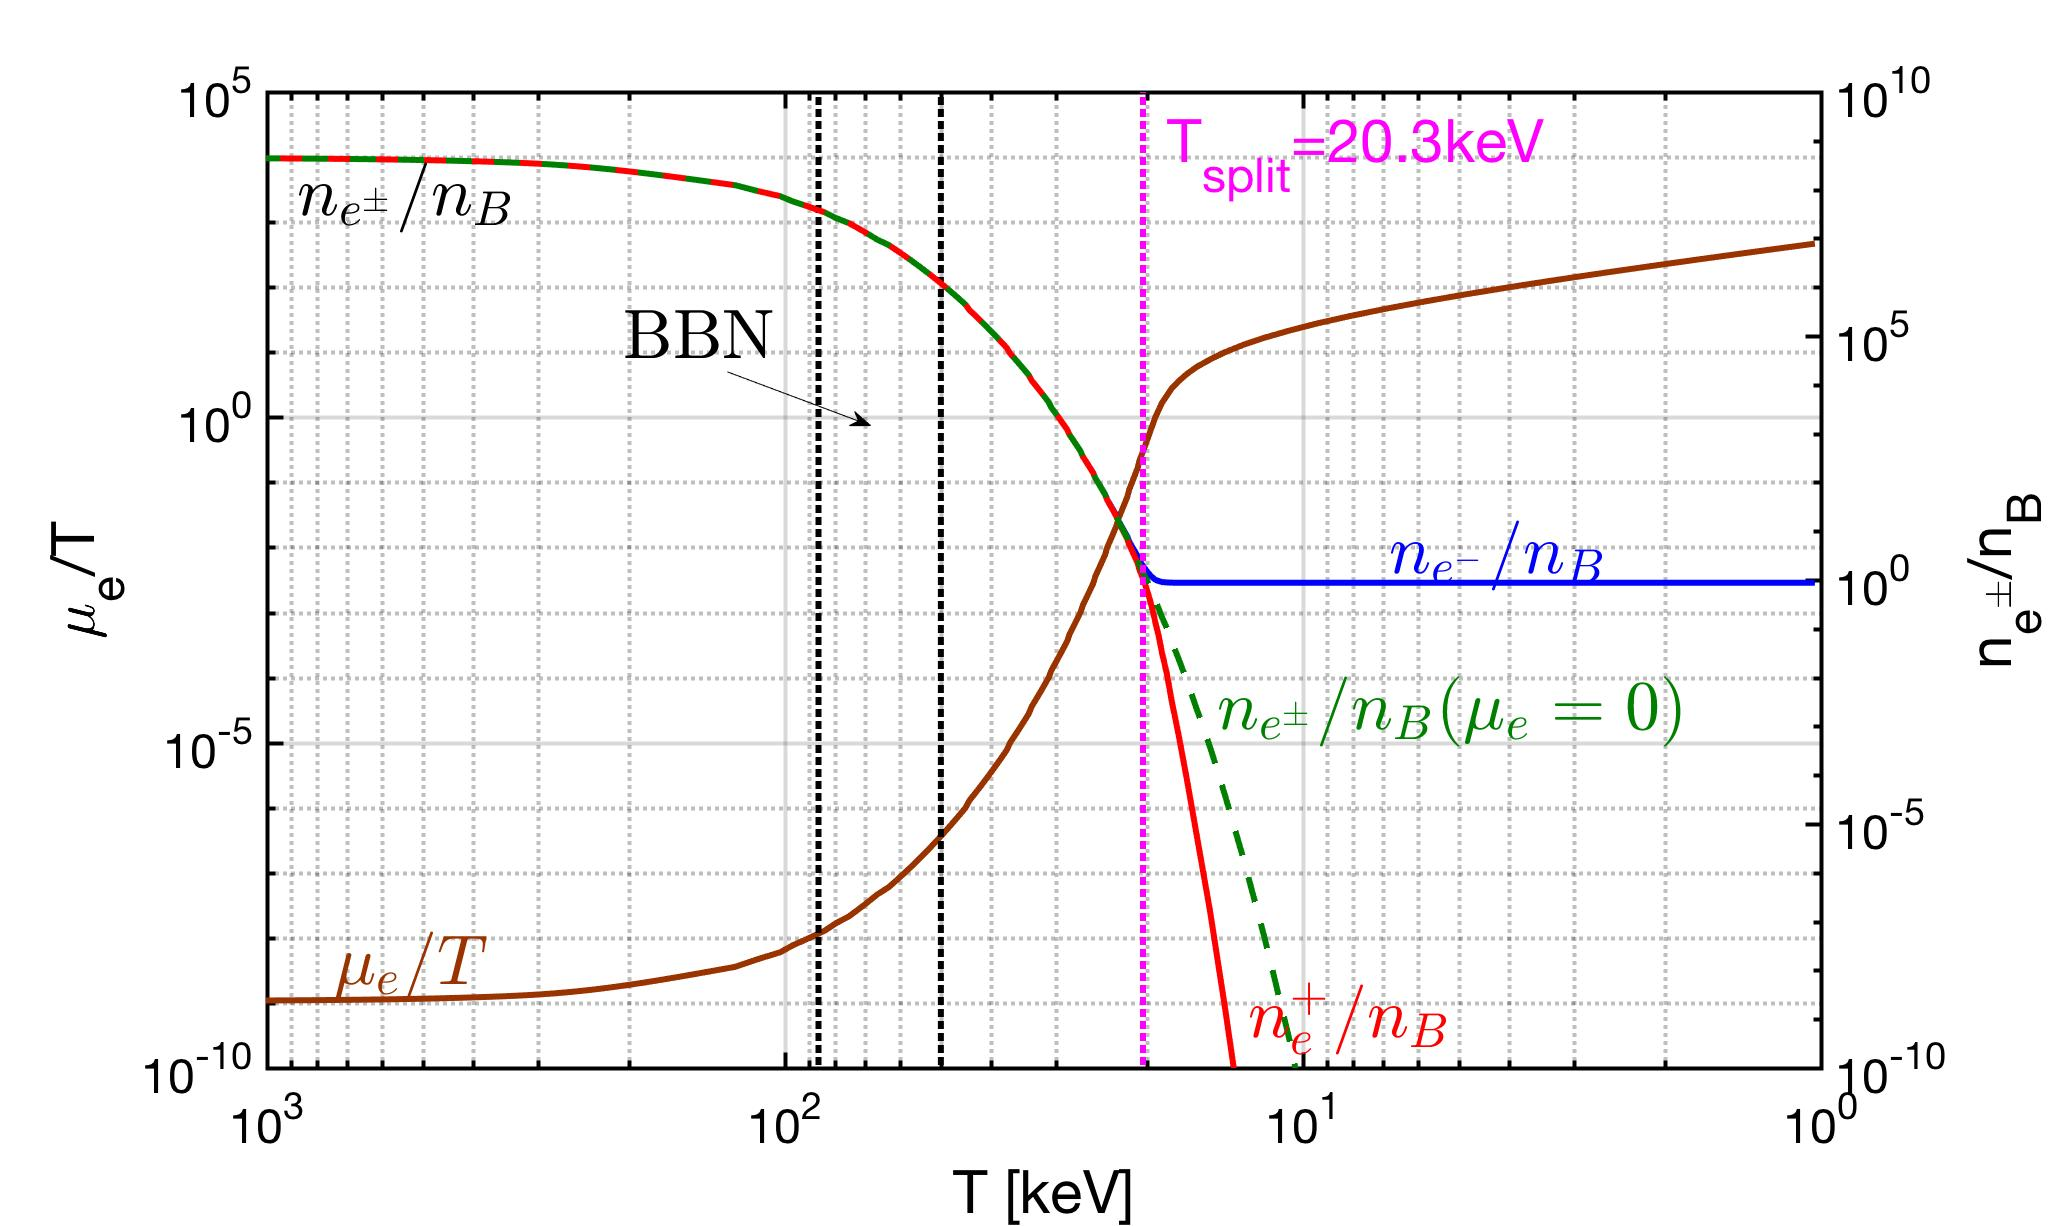
\includegraphics[width=0.95\linewidth]{plots/chap03BBN/May152023_EPDensity_Chemical}
% \caption{Left axis: The chemical potential of electrons as a function of temperature by numerically solving Eq. (\ref{charge_neutral_cond3}) with $n_p/n_B=0.878$ and $n_B/n_\gamma=6.05\times10^{-10}$. Right axis: the ratio of electron (positron) number density to baryon density as a function of temperature. The solid blue line is the electron density, the red dashed line is the positron density, and the green dotted line is the number density with $\mu_e=0$. When $T=20.3\,\mathrm{keV}$ (the purple vertical line) positron density decreases rapidly because of the annihilation. The vertical black dotted lines represent BBN temperature range $86\,\mathrm{keV}>\mathrm{T_{BBN}}>50\,\mathrm{keV}$.}
% \label{BBN_Electron}
% \end{center}
% \end{figure}
%~~~~~~~~~~~~~~~~~~~~~~~~~~~~~~~~~~~~~~~~~~~~~~~~~~~~~

% In Fig.~\ref{BBN_Electron} (left axis), we solve Eq.~(\ref{charge_neutral_cond3}) numerically and plot the electron chemical potential as a function of temperature with the following parameters: proton concentration $X_p=0.878$ from observation~\cite{ParticleDataGroup:2022pth} and $n_B/n_\gamma=6.05\times10^{-10}$ from CMB. We can see the value of chemical potential is comparatively small $\mu_e/T\approx10^{-6}\sim10^{-7}$ during the BBN temperature range, implying an equal number of electrons and positrons in plasma. The ratio of electron (positron) number density to baryon density shows that the Universe was filled with an electron-positron rich plasma during the accepted BBN temperature range. For example, when the temperature is around $T=70\,\mathrm{keV}$, the density of electrons and positrons is comparatively large $n_{e^\pm}\approx10^7\,n_B$. At $90$\,keV, the electron and positron density is near the solar core density, see Fig.~19 in Ref.~\cite{Rafelski:2023emw}. Later when the temperature is around $T=20.3\,\mathrm{keV}$, the positron density decreases, transforming the pair-plasma to an electron-baryon plasma.


%%%%%%%%%%%%%%%%%%%%%%%%%%%%%%%%%%%%%%%%%%%%%%%%%%%%%
%\subsubsection\label{sec:relax}
\paragraph{The damping rate in electron-positron plasma:}
To find the damping rate in the BBN electron-positron plasma, we considered the major scatterings between photons and $e^+e^-$ pairs: inverse Compton scattering, M{\o}ller scattering, and Bhabha scattering
\begin{align}
&e^\pm+\gamma\longrightarrow e^\pm+\gamma,\qquad e^\pm+e^\pm\longrightarrow e^\pm+e^\pm,\qquad e^\pm+e^\mp\longrightarrow e^\pm+e^\mp\,.
\end{align}
% In general, to evaluate the reaction rate in two-body reaction $1+2\rightarrow3+4$ in the Boltzmann approximation we can use reaction cross-section $\sigma(s)$ and the relation from Ref.~\cite{Letessier:2002ony}:
% \begin{align}\label{GeneralRate}
% R_{12\rightarrow34}=\frac{g_1g_2}{32\pi^4}\frac{T}{1+I_{12}}\!\!\int^\infty_{s_{th}}\!\!\!\!ds\,\sigma(s)\frac{\lambda_2(s)}{\sqrt{s}}\!K_1\!\!\left({\sqrt{s}}/{T}\right),
% \end{align}
% where $K_1$ is the first-order Bessel function and the K\"{a}ll\'{e}n function $\lambda_2(s)$ is defined as
% \begin{align}
% \lambda_2(s)=\left[s-(m_1+m_2)^2\right]\left[s-(m_1-m_2)^2\right],
% \end{align}
% with $m_{1/2}$ and $g_{1/2}$ are the masses and degeneracies of initial interacting particles. The factor $1/(1+I_{12})$ is introduced to avoid double counting of indistinguishable pairs of particles, we have $I_{12}=1$ for identical particles and $I_{12}=0$ otherwise. 

% The two-body cross-section can be obtained by averaging the matrix element over the Mandelstam variable $t$. We have
% \begin{align}
% &\sigma_{e^\pm\gamma}=\frac{1}{16\pi(s-m_e^2)^2}\int^0_{-(s-m_e^2)^2/s}\!\!\!\!\!\!\!\!\!\!\!\!\!\!\!\!\! dt\, |M_{e^\pm\gamma}|^2,\\
% &\sigma_{e^-e^-}=\frac{1}{16\pi s(s-4m_e^2)}\int^0_{-(s-4m_e^2)}\!\!\!\!\!\!\!\!\!\!\!\!\!\!\!\!\!dt\, |M_{e^\pm e^\pm}|^2,\\
% &\sigma_{e^-e^+}=\frac{1}{16\pi s(s-4m_e^2)}\int^0_{-(s-4m_e^2)}\!\!\!\!\!\!\!\!\!\!\!\!\!\!\!\!\!dt\, |M_{e^\pm e^\mp}|^2.
% \end{align}
% The matrix element associated with inverse Compton scattering is given by~\cite{Kuznetsova:2009bq, Kuznetsova:2011wt}
% \begin{align}
% |M_{e^\pm\gamma}|^2\!&=32 \pi^2\alpha^2\bigg[4\left(\frac{m_e^2}{m_e^2-s}+\frac{m_e^2}{m_e^2-u}\right)^2\notag\\
% & -\frac{4m_e^2}{m_e^2-s}-\frac{4m_e^2}{m_e^2-u} -
% \frac{m_e^2-u}{m_e^2-s} -\frac{m_e^2-s}{m_e^2-u}\bigg],
% \end{align}
% and for M{\o}ller and Bhabha scattering we have respectively
% \begin{align}
% &|M_{e^{-}e^{-}}|^{2}\!=64\pi^{2}\alpha^{2}\bigg[
% \frac{s^{2}+u^{2}+8m_e^{2}(t-m_e^{2})}{2(t-m^2_{\gamma})^{2}} \notag\\ 
% &+\frac{{s^{2}+t^{2}}+8m_e^{2}
% (u-m_e^{2})}{2(u-m_{\gamma}^2)^{2}} + \frac{\left( {s}-2m_e^{2}\right)\left({s}-6m_e^{2}\right)}
% {(t-m_{\gamma}^2)(u-m_{\gamma}^2)} \bigg],
% \end{align}
% and
% \begin{align}
% &|M_{e^- e^+}|^{2}=64\pi^{2}\alpha^{2}
% \bigg[\frac{s^{2}+u^{2}+8m_e^{2}(t-m_e^{2})}{2(t-m^2_{\gamma})^{2}}\notag\\
% &+\frac{u^{2}+t^{2}+8m_e^{2}
% (s-m_e^{2})}{2(s-m^2_{\gamma})^{2}} + \frac{\left({u}-2m_e^{2}\right)\left({u}-6m_e^{2}\right)}
% {(t-m^2_{\gamma})(s-m^2_{\gamma})} \bigg],
% \label{M_fi_b}
% \end{align}
% where $s, t, u$ are the Mandelstam variables and we included the photon mass $m_\gamma$ to avoid singularity in reaction matrix elements. The photon mass in plasma is equal to the plasma frequency, in our case we have~\cite{Kislinger:1975uy}
% \begin{equation}
% m^2_\gamma=\omega^2_{p}=8\pi\alpha\int\frac{d^3p_e}{(2\pi)^3}\left(1-\frac{p_e^2}{3E_e^2}\right)\frac{f_- +f_+}{E_e},
% \end{equation}
% where $f_-$ and $f_+$ are the single-particle distribution functions for electrons and positrons respectively, and $E_e=\sqrt{p_e^2+m^2_e}$ is the electron energy. In the BBN temperature range $m_e\gg T$ and if we consider the non-relativistic electron and positron plasma
% \begin{align}
% m^2_\gamma=\frac{4\pi\alpha}{2m_e}\left(\frac{2m_eT}{\pi}\right)^{3/2}e^{-m_e/T}\cosh\left(\frac{\mu_e}{T}\right).
% \end{align}

% Substituting the cross-sections into Eq.~(\ref{GeneralRate}), the thermal reaction rate per volume for inverse Compton scattering can be written as
% \begin{align}
% R_{e^\pm\gamma}=\frac{g_eg_\gamma}{16\left(2\pi\right)^5}T\int_{m_e^2}^\infty\!\!\!\!ds\frac{K_1(\sqrt{s}/T)}{\sqrt{s}}\int^0_{-(s-m_e^2)^2/s}\!\!\!\!\!\!\!\!\!\!\!\!\!\!\!\!\!\!\!\!\!\!dt\, |M_{e^\pm\gamma}|^2,
% \end{align} 
% for M{\o}ller and Bhabha scattering we have
% \begin{align}
% &R_{e^\pm e^\pm}=\frac{g_eg_e}{16\left(2\pi\right)^5}T\!\!\int_{4m_e^2}^\infty\!\!\!\!ds\frac{K_1(\sqrt{s}/T)}{\sqrt{s}}\int^0_{-(s-4m_e^2)}\!\!\!\!\!\!\!\!\!\!\!\!\!\!\!\!\!\!\!\!\!\!dt\,|M_{e^\pm e^\pm}|^2,\\
% &R_{e^\pm e^\mp}=\frac{g_eg_e}{16\left(2\pi\right)^5}T\!\!\int_{4m_e^2}^\infty\!\!\!\!ds\frac{K_1(\sqrt{s}/T)}{\sqrt{s}}\int^0_{-(s-4m_e^2)}\!\!\!\!\!\!\!\!\!\!\!\!\!\!\!\!\!\!\!\!\!\!dt\,|M_{e^\pm e^\mp}|^2.
% \end{align}
\begin{figure}[h!]
\begin{center}
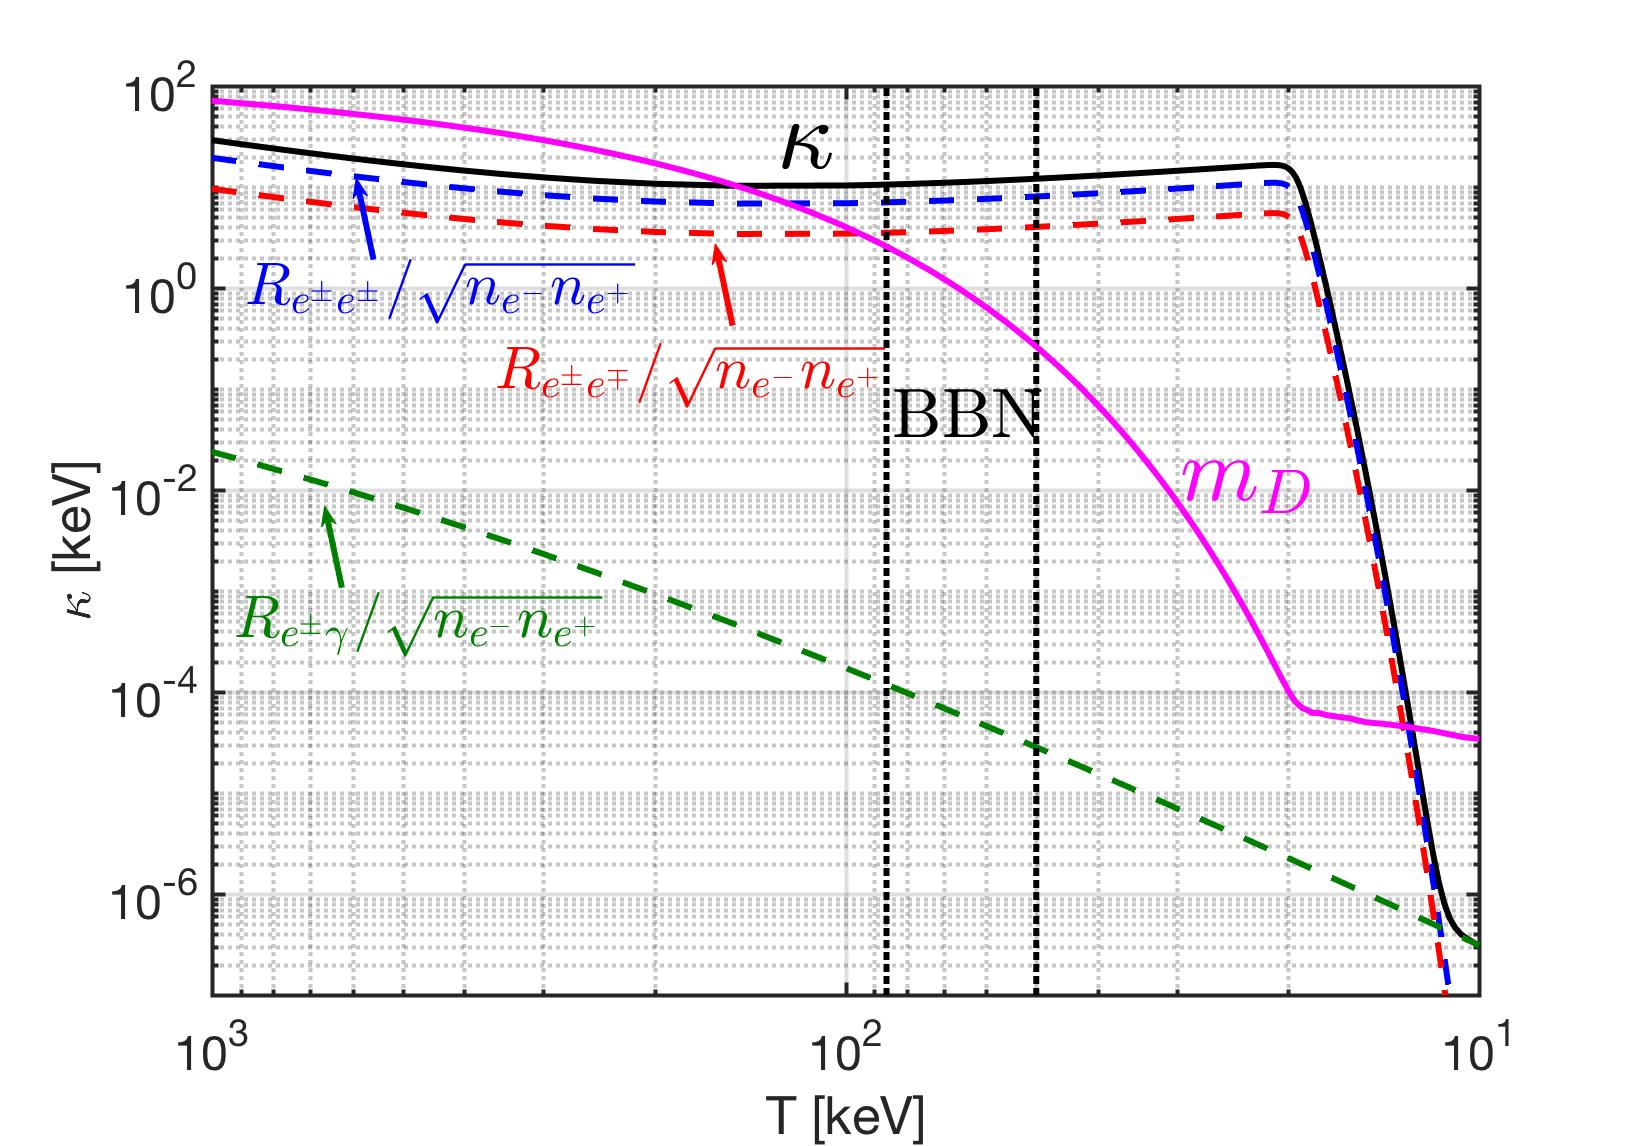
\includegraphics[width=0.95\linewidth]{plots/chap03BBN/May152023Kappa_EPPlasma002}
%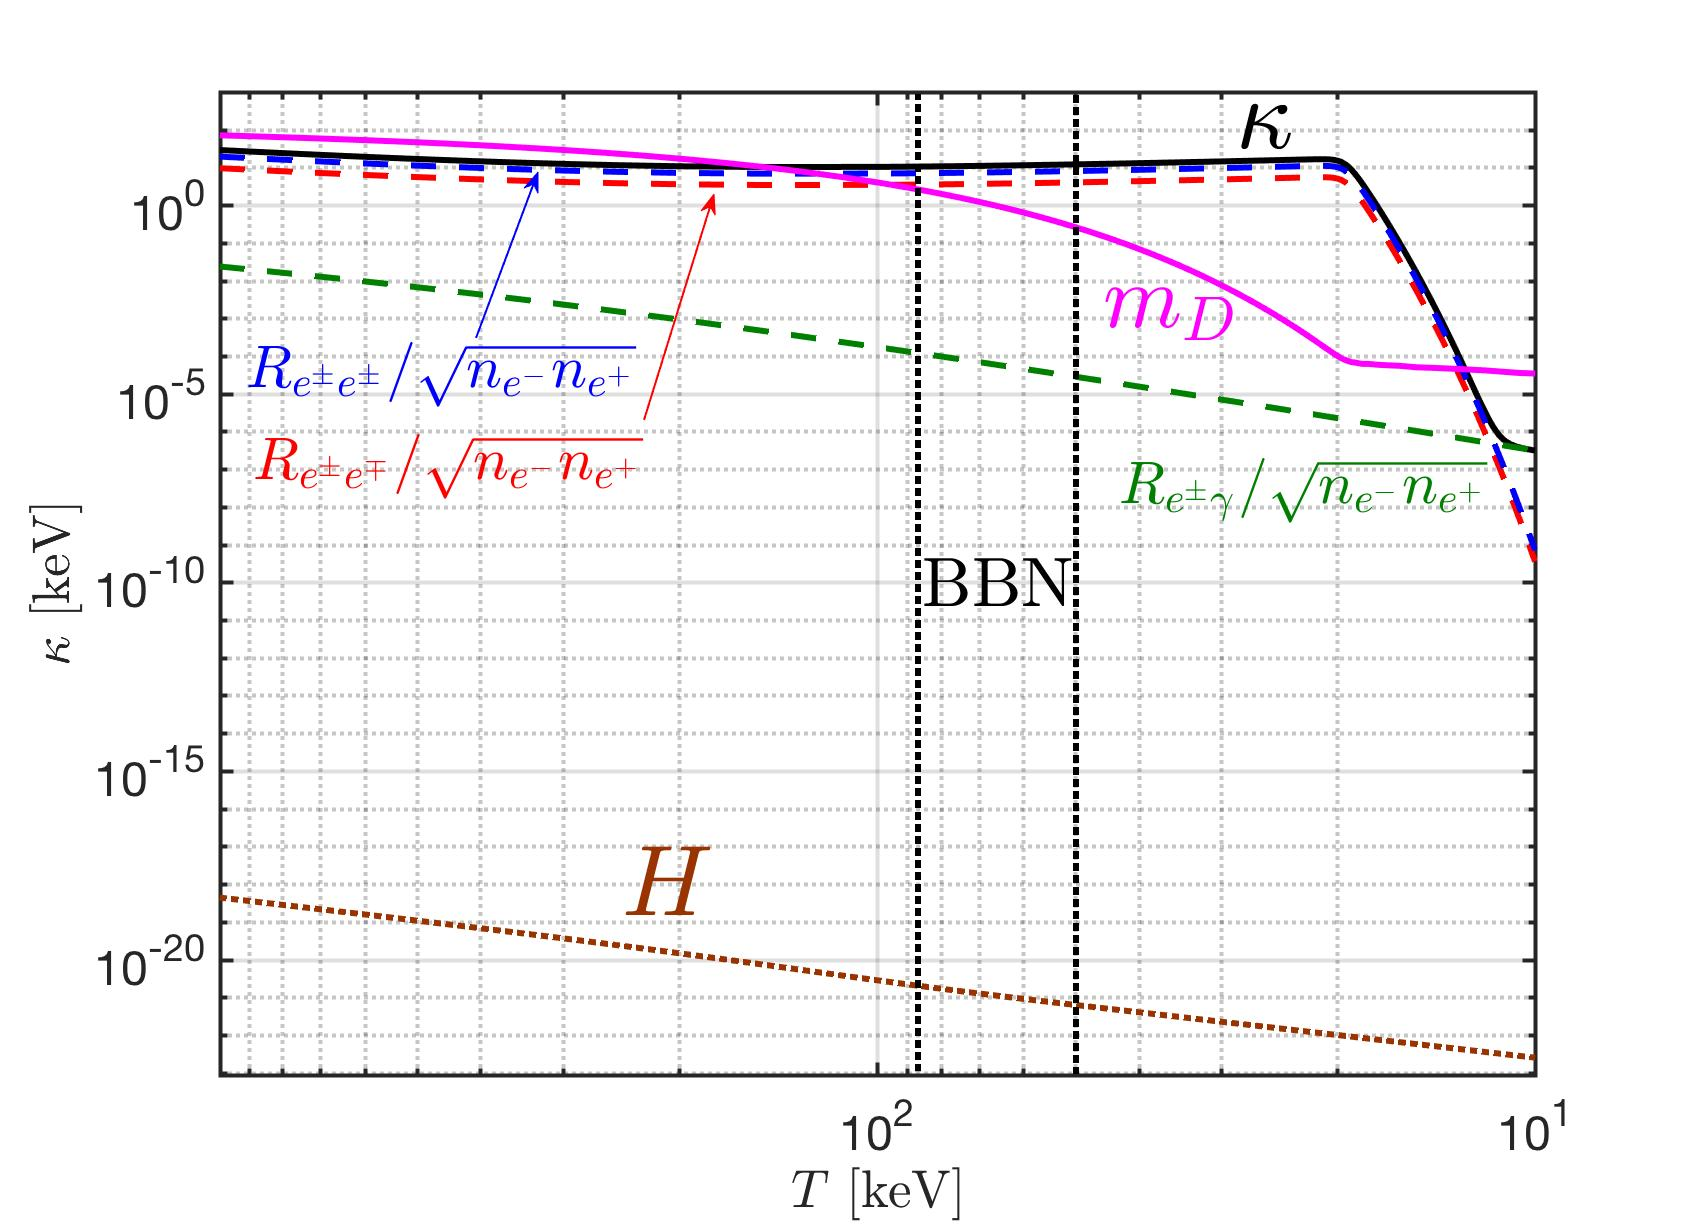
\includegraphics[width=0.95\linewidth]{May152023Kappa_EPPlasma}
\caption{\cccite{Grayson:2023flr}, adapted from Ref.~\cite{Grayson:2023flr} and thesis of C.T.Yang \cite{Yang:2024ret}. The relaxation rate $\kappa$ as a function of temperature in non-relativistic electron-positron plasma. We present reaction rates for M{\o}ller scattering $R_{e^\pm e^\pm}$ (blue dashed line), Bhabha scattering $R_{e^\pm e^\mp}$ (red dashed line), and inverse Compton scattering $R_{e^\pm \gamma}$ (green dashed line). The average relaxation rate from Eq.~(\ref{Kappa}) is shown as a black solid line. The vertical black dotted lines represent BBN temperature range $86\,\mathrm{keV}>\mathrm{T_{BBN}}>50\,\mathrm{keV}$ during which the average relaxation rate is $\kappa=10\sim12$ keV. The dominant reactions during BBN are the M{\o}ller and Bhabha scatterings. The purple solid line represents the Debye mass given by Eq.~(\ref{eq:mL})}.
\label{RelaxationRate_fig}
\end{center}
\end{figure}
C. T. Yang calculated these reaction rates by considering in-plasma tree-level QED scatterings using an infrared cutoff at $\omega_p$, which is the temperature-dependent effective photon mass in a plasma \cite{Yang:2024ret}.
In Fig.~\ref{RelaxationRate_fig}, we show the reaction rates $R$ for M{\o}ller, Bhabha, and inverse Compton scattering as a function of temperature. For temperatures $T>12.0$ keV, the dominant reactions in plasma are M{\o}ller and Bhabha scatterings between electrons and positrons. Thus, we can neglect the inverse Compton scattering in the BBN temperature range.
We then use these scattering rates in plasma to find the average damping rate:
\begin{align}\label{Kappa}
\kappa=\frac{R_{e^\pm e^\pm}+R_{e^\pm e^\mp}+R_{e^\pm\gamma}}{\sqrt{n_{e^-}n_{e^+}}}\approx\frac{R_{e^\pm e^\pm}+R_{e^\pm e^\mp}}{\sqrt{n_{e^-}n_{e^+}}},
\end{align}
where we neglect the inverse Compton scattering during BBN as discussed. The density function ${\sqrt{n_{e^-}n_{e^+}}}$ in the Boltzmann limit is given by
\begin{align}
{\sqrt{n_{e^-}n_{e^+}}}=\frac{g_e}{2\pi^3}T^3\left(\frac{m_e}{T}\right)^2K_2(m_e/T).
\end{align}
In Fig.~\ref{RelaxationRate_fig} that the total damping rate $\kappa$ given by Eq.~(\ref{Kappa}) is approximately constant $\kappa=10-12$ keV during the BBN. This value is much larger than the Debye mass defined below in Eq.~(\ref{eq:mL}). Below $T<20.3$ keV, the relaxation rate $\kappa$ decreases rapidly because the positrons disappear. At $T=12$\,keV, the inverse Compton scattering of remaining electrons becomes the dominant scattering process. 

\subsection{Electron positron plasma screening in BBN}\label{sec:Discussion}

In this chapter, we review \cite{Grayson:2023flr}, which applies the non-relativistic longitudinal polarization function to study the dynamics of the electron-positron plasma in the early Universe. In particular, we discussed the damping rate, the electron-positron to baryon density ratio, and their potential implications for Big Bang Nucleosynthesis (BBN) through screening within linear response theory. We derived an approximate analytic formula for the potential of a moving heavy charge in a collisional plasma in \req{eq:pos_point_DDS} describing screening effects previously found only numerically \cite{Hwang:2021kno}. Our analytic formula can be readily used to estimate the effect of screening on thermonuclear reactions using \req{eq:DDSenhance}. The correction to thermonuclear reactions due to damped-dynamic screening is small due to the low velocity of nuclei and a large amount of collisional scattering. This is in line with the findings of \cite{Hwang:2021kno}, who conclude that even though the densities are large, they are not enough to modify the potential at short distances related to screening. The analytic expression we find for the nuclear reaction rate enhancement \req{eq:DDSenhance} in a collisional plasma could be useful in other fusion environments such as stellar fusion and laboratory fusion experiments, such as those discussed in ~\cite{Labaune:2013dla,Margarone:2022mdpi}.

Overall we were very surprised to find that the screening effects in BBN were so small even in the static case, considering that the number densities present during BBN are $\sim 10^4$ times normal matter. If we compare this to screening effects on Earth, we can see that although plasmas occur at lower densities, they also occur in much colder environments. The strength of the screening effect is related to the Debye mass
\begin{equation}
m_D^2 \sim \frac{n_\text{eq} }{T}\,,
\end{equation}
which is on the order of a few keV during BBN. On earth, $n_\text{eq}$ is decreased by $\sim 10^4$, but T is decreased by $\sim 10^6$. Thus, we would expect to see similar, if not larger, screening effects on Earth. For instance, the Debye screening length in extracellular fluid in the body is 8 \AA ngstrom \cite{Wennerstrom:2020}, only a factor of $\sim 20$ times larger than the Debye length during BBN. We can have these large densities at low temperatures on earth due to gravity's agglomeration of matter in the universe.
\subsection{The short-range screening potential}
In \cite{Grayson:2023flr}, a proposal is made to study the short-range potential relevant to quantum tunneling in thermonuclear reactions. Since the Gamow energy at which nuclei are most likely to tunnel is above the thermal energy, the portion of the screening potential relevant for tunneling does not satisfy the "weak-field" limit where the electromagnetic energy is small compared to the thermal energy
\begin{equation}
 \frac{q \phi(x)}{T} \ll 1\,.
\end{equation}
When this condition is not satisfied one must consider the full equilibrium distribution when calculating the short-range potential \cite{Hakim:1967prd,DeGroot:1980dk}
\begin{equation}\label{eq:Boltz}
 f_B^\pm(x,p) = e^{-(p_0\pm e\phi(x))/T}\,.
\end{equation}
The $e\phi$ term in the exponential accounts for the change in energy of a charge in the plasma due to its presence in an external field. For this equilibrium distribution, a linear response is no longer possible since the equilibrium distribution depends on the external electromagnetic field. In equilibrium one can find the static screening potential for strong electromagnetic fields using the nonlinear Poisson-Boltzmann equation,
\begin{equation}\label{eq:Poisson-Boltz}
 -\nabla^2 e\phi_{(\text{eq})}(x)/T +m_D^2\sinh\left[e\phi_{(\text{eq})}(x)/T\right] =e\rho_\mathrm{ext}(x)/T\,.
 \end{equation}
This equation has a well-known solution for an infinite sheet which we used to argue the importance of strong screening in BBN. 
In a future publication, we will solve the Poisson-Boltzmann equation with strong screening to calculate the short-range screening potential in BBN. We note that the toy model in \cite{Grayson:2023flr} overestimates strong screening effects for two reasons: an infinite sheet has a constant electric field requiring more polarizing charge density to screen the field, and the Boltzmann distribution in \req{eq:Boltz} does not account for the stacking of electron-positron states when the density of electrons and positrons becomes very large near the nucleus. Both of these effects significantly reduce the effect of strong screening on reaction rates, but at the time of writing, it seems that strong screening will create a larger effect on nuclear reaction rates than damped-dynamic screening. Predicting enhanced screening may be relevant for the anomalous screening observed in the measurements of astrophysical S(E) factors \cite{Zhang:2020nuc}.

%%%%%%%%%%%%%%%%%%%%%%%%%%%%%%%%%%%%%%%
\subsubsection{Dusty plasmas}
In \cite{Grayson:2023flr} were very interested in finding BBN plasma had similar properties to planetary and space dusty plasma theory~\cite{Montgomery:1970jpp,Stenflo:1973,Shukla:2002ppcf,Lampe:2000pop}. The large distance behavior of the damped-dynamic BBN screened potential in \req{eq:pos_point_DDS} matched that of slowly moving dust particles in plasma \cite{Stenflo:1973}. Dusty plasma theory studies many effects not currently included in BBN plasma studies, including dust charging, dust acoustic waves, dust instabilities, and structure formation (dust crystals)~\cite{Shukla:2002ppcf}. We expect that these results can be ported to the nuclear light element dust dynamics in the primordial $e^-e^+\gamma$ QED plasma. This interdisciplinary connection, which has not been recognized previously, could have substantial implications for our understanding of the evolution of matter in the early Universe.

%%%%%%%%%%%%%%%%%%%%%%%%%%%%%%
\subsubsection{Structure formation in the early universe}
One may note that the portion of the screening potential in the direction of motion is slightly binding \reff{fig:dynamiclinear}.
Given recent observations from JWST \cite{Ferreira:2023jwst}, one could speculate that this polarization binding effect could lead to the early seeding of matter structure in the Universe. In dusty plasmas, this happens due to an attractive portion of the internuclear (charged dust) potential, which favors a specific average separation between charged dust particles. From the plasma parameters calculated in \cite{Grayson:2023flr} the depth of the binding potential is on the order of 10's of electron volts. While this is more energy than the usual molecular bond, the BBN temperature is likely too large for these binding energies to play a role in dynamics. Given the potential in \req{eq:pos_point_DDS}, calculating if a molecular bound state exists is the subject of future work.
%%%%%%%%%%%%%%%%%%%%%%%%%%%%%%%%


\section{Summary and Outlook}
\label{sec:SummOut}
THIS IS FOR LAST SECTION COLLECTION OF MATERIAL NOT FIT TO USE IN INTRO

\subsubsection{QGP in the early universe}
 QGP filled the universe  after the Big Bang \cite{Rafelski:2013yka}. One could study the QCD potential of heavy quarks propagating through QGP in heavy ion collisions or the early universe. In dynamic screening of heavy quarks, it is possible that a long-range attractive potential also arises, leading to the formation of inhomogeneities in the early universe during the QGP epoch. In QCD, the transport equations are complicated by their non-abelian nature. Since gluons can couple to the external field of heavy quarks, they would contribute non-trivially to the transport equations. We expect we would also have to use strong-field kinetic theory due to the large QCD coupling $\alpha_s$. Kinetic theory in QGP is discussed in detail in \cite{Mrowczynski:2016etf}.
%%%%%%%%%%%%%%%%%%%%%%%%%%%%%%%%%%%%%%%%%%%%%%%%%%%%%%%%%%%%%%%%%%%
% {Composition
%%%%%%%%%%%%%%%%%%%%%%%%%%%%%%%%%%%%%%%%%%%%%%%%%%%%%%%%%%%%%%%%%%%%%%